\chapter{Appendix}

\begin{figure}
	\centering
	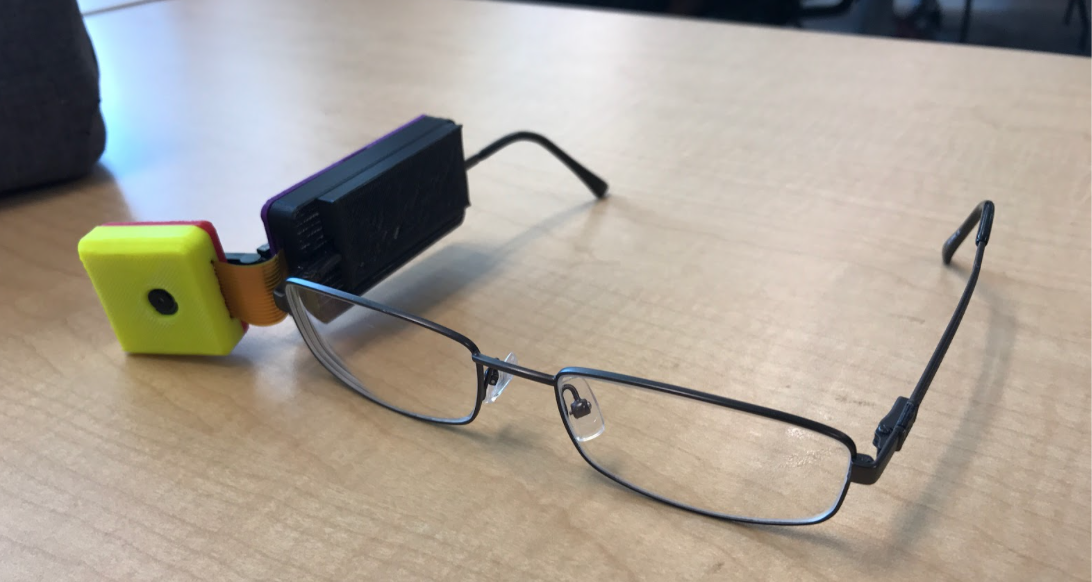
\includegraphics[scale = 0.5]{PRAHVI-HARDWARE}
	\caption{Hardware}
	\label{headsetPic}
\end{figure}

\begin{figure}
	\centering
	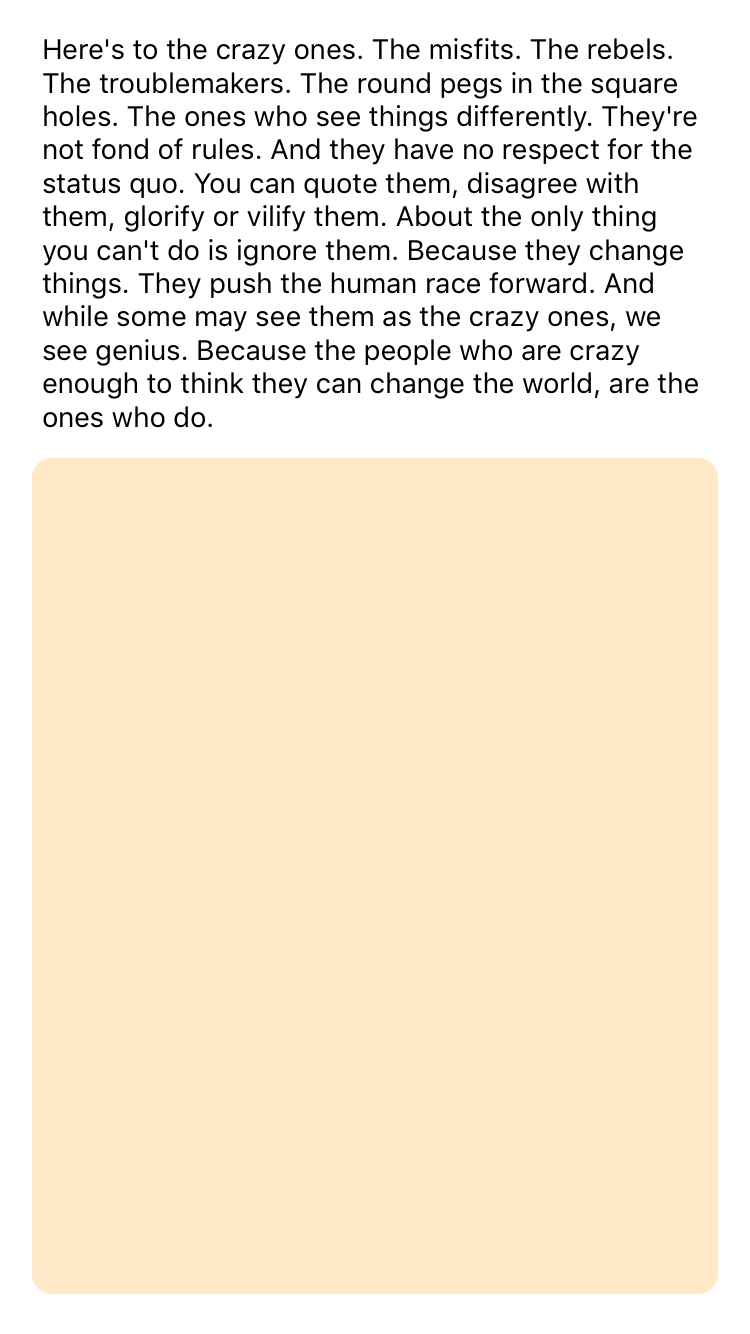
\includegraphics[scale = 0.2]{ui}
	\caption{User Interface}
	\label{uipicture}
\end{figure}

\pagebreak

\section{Sample Testing Documents}
\subsection{Can Amazon's assistant stay on top?}
http://www.bbc.com/news/technology-39853718
\subsubsection{Original Text}
Amazon surprised everyone when, in late 2014, it unveiled a standalone digital assistant that was not only good, but blew away the competition in both quality and aesthetics.
The Echo - a cylindrical speaker with microphone - now accounts for just over 70\% of all digital assistant use in the US, leaving its nearest competitor, Google Home, well behind.
It's an important new market, even if the idea of talking to an object in your home still comes uneasily to many of us.
In a new report, Emarketer estimated 36 million Americans will use a voice-activated assistant at last once a month - an increase of 129\% on this time last year.
Amazon, as I mentioned, already has the lion's share. It's now hoping to echo (sorry) that success with its latest effort which we could see as early as Tuesday, according to reports.
AFTV.com, a site with a solid track record of leaks, said it found a low-quality image of the device on Amazon's own servers.
The authenticity of the image was later backed up by king-of-the-leaks, Evan Blass. 
The new device is expected to house a 7-inch touchscreen and can be used for video calling, as well as displaying weather information and other data.
It will help plug that gap that many voice assistant users will be familiar with, like not knowing how long a timer has left without asking. Or just knowing the time - it's a step backwards to not just look at a clock. Of course, a screen opens up a range of new possible interactions.
'Barely crossed the starting line'
Dominating this area isn't just about selling assistants. The opportunity for Amazon here is in an arena few thought they become a major player - home automation. Emarketer's data suggests that once you opt for one brand of assistant in your home, you're very unlikely to jump ship. So when the "internet of things" boom finally hits (any day now, as we've been saying the past three years) Amazon's early lead could really start to pay off.
Or, it could blow it. Consider Amazon's lead like doing well in the first event of a heptathlon.
"Amazon has a head start in the voice race but the industry has barely crossed the starting line," said CCS Insight analyst Geoff Blaber. I caught him as he was on his way to Microsoft's developer's conference, where its own digital assistant, Cortana, will be centre stage.
He added: "Those that can maximize customer data, search, artificial intelligence and natural language processing, make it all available to developers to innovate with, and simultaneously walk the privacy tightrope, will be the ultimate winners."
As it seeks to rapidly expand its lead, Amazon has made itself incredibly developer-friendly compared to its rivals. I recently had a spin in an Alexa-enabled Ford, and General Electric today announced an Alexa-powered lamp. Amazon wants Alexa in as many nooks and crannies of our lives as possible.

\subsubsection{Detected Text}
Amazon surprised everyone when. in late 2014. it unveiled a standalone diaitat assistant
that was not only good. but blew away the competition in both quality and aesthetics.
The ticho - a eytindrical speaker with microphone - now accounts for just over 70\%6 of all
Jurital ausistant use in the US, leaving its nearest competitor, Google Home, well behind.
\#'s an important new market, even if the idea of talking to an object in your home still
comes uneasity to many of us
in a new report, Emarketer estimated 36 million Americans will use a voice-activated
at last once a month - an increase of 129\% on this time last year
Amazon, as I mentioned. already has the lion's share, It's now hoping to echo (sorry) that
with its latest effort which we could see as early as Tuesday. according to reports
AIPTV.com, a site with a soild track record of leaks, said it found a low-quality image of the
device on Amazon's own servers.
The authenticity of the image was later backed up by king-of the- leaks. Evan
"The new device is expected to house a 7-inch touchscreen and can be used for video calling.
as well as displaying weather information and other data:
It will help plug that wap that many voice assistant users will be familiar with. like not
knowing how long a timer has left without asking. Or Just knowing the time -it's a step
backwards to not just look at a clack. Of course. a screen opens up a range of new possible
interactions.
"tarely croused the starting tine"
Dominating this area isn't just about selling assistants, The opportunity for Amazon here is
in an arena few thought they became a major player - home automation. Emarketer's data
sumrests that once you opt for one brand of assistant in your home. you're very unlikely to
Jurnp ship. So when the "internet of things" boom finally hits (any day nowe as we've been
saying the past three years) Amazon's early lead could really start to pay off.
Or it could blow it. Consider Amazon's lead like doing well in the first event of a heptathlon.
"Amazon has a head start in the vaice race but the industry has barely crossed the starting
line." said CCS Insight analyst Geoff caught him as he was on his way to Microsoft's
(developer's conference. where its own digital assistant, Cortana, will be centre stage:
He added: "Those that can maximize customer data, yearch, artificial intelligence and
natural language processing. make it all available to developers to innovate with. and
simultancousty walk the privacy tightrope. will be the ultimate winners."
As it seeks to rapidly expand its ead. Amazon has made itself incredibly developer-triendy
compared to its rivals I recently had 'a spin in an Alexa-enabled Ford. and General Electric
today announced an Alexa-powered lamp. Amazon wants Alexa in as many nooks and
crannies of our tives as possible.
t

\subsection{Dubai becomes first city to get its own Microsoft font}
http://www.bbc.com/news/business-39767990
\subsubsection{Original Text}
Not content with having the world's tallest building and biggest shopping centre, Dubai has become the first city to get its own Microsoft-designed font.
The typeface comes in both Latin and Arabic script, and will be available in 23 languages.
Government bodies have been told to use it in official correspondence.
But given the human rights record of Dubai and the United Arab Emirates, eyebrows will be raised at claims it is a font of "self-expression".
'Create harmony'
Dubai's Crown Prince Hamdan bin Mohammed al-Maktoum said he had been personally involved in "all the stages" of the development of the font.
It was "a very important step for us as part of our continuous efforts to be ranked first in the digital world," he added.
"We are confident that this new font and its unique specifications will prove popular among other fonts used online and in smart technologies across the world".
Dubai's government said the typeface's design "reflects modernity and is inspired by the city" and "was designed to create harmony between Latin and Arabic".
When self expression isn't usually your type
"Self-expression is an art form," says the blurb accompanying the launch of this font.
"Through it you share who you are, what you think and how you feel to the world. To do so you need a medium capable of capturing the nuances of everything you have to say.
"The Dubai Font does exactly that. It is a new global medium for self-expression."
But the United Arab Emirates - of which Dubai is part - has been criticised for its restrictions on free speech.
The constitution does guarantee the right to freedom of opinion and expression, but Human Rights Watch (HRW) says this "has no effect on the daily life of the citizen" and the country "has seen a wave of arrests and violations of human rights and freedoms and mute the voices of dissent".
In March, high-profile human rights activist Ahmed Mansoor was arrested, a move HRW said showed "complete intolerance of peaceful dissent".
The UAE's official news agency, WAM, said Mr Mansoor had been held "on suspicion of using social media sites to publish "flawed information" and "false news" to "incite sectarian strife and hatred" and "harm the reputation of the state."

\subsubsection{Detected Text}
Not content with having the world i tallest building and best shopping centre, Dubai has
become the first city to get its own Microsoft designed font:
"The typeface comes in both Latin and Arabic script. and will be available in 23 languages.
Government bodies have been told to use it in official correspondence
Wat aiven the human rights record of Dubai and the United Arab Emirates. eyebrows will be
raised at claim it in a font of "welt-expression".
'Create harmony
Bubal's Grown Prince Hamdan bin Mohammed al- Maktoum said he had been personally
involved in "all the stages" of the development of the font.
It was "a very important step for us as part of our continuous efforts to be ranked first in
the world he added.
"We are confident that this new font and its unique specifications will prove popular among
other fonts used ontine and in smart technologies across the world".
Dubai's government said the typeface's destin "reflects modernity and is inspired by the
vity" and "was destined to create harmony between Latin and Arabic'.
When self expression isn't usually your type
"Seit exnression is an art form" says the blurb accompanying the launch of this font.
"Ihrough it you share who you are. what you think and how you feel to the world. To do so
you need a medium capable of capturing the nuances of everything you have to say.
"Ime Dubai Font does exactly that. it is a new global medium for self-expression."
hat the United Arab Emirates - of which Duba is part - has been criticised for its
restrictions on tree speech
"The constitution does nuarantee the right to freedom of opinion and expression. but Human
Wights Watch (HRW) says this "has no effect on the daily life of the citizen" and the country
"has ween a wave af arrests and violations of human rights and freedoms and mute the
voices of dissent
\\n March: high profile human rights activist Ahmed Mansoor was arrested, a move HRW
said showed "compete intolerance of peaceful dissent~;
The UAE's official news agency: WAM, maid Mr Manzoor had been held "on suspicion of
using social media sites to publish "flawed information" and "false news" to "incite
sectarian strife and hatred" and "harm the reputation of the state."

\subsection{FCC website 'targeted by attack' after John Oliver comments}
http://www.bbc.com/news/technology-39855490
\subsubsection{Original Text}
The US Federal Communications Commission (FCC) website was deliberately attacked on 8 May, the regulator has said.
The incident began hours after comedian John Oliver criticised FCC plans to reverse US net neutrality rules.
Mr Oliver urged people to post to the site's online commenting system, protesting against the proposals.
The FCC said that issues with the site were caused by orchestrated attacks, not high volumes of traffic.
"These actors were not attempting to file comments themselves; rather they made it difficult for legitimate commenters to access and file with the FCC," chief information officer Dr David Bray said in an official statement.
"While the comment system remained up and running the entire time, these distributed denial of service (DDoS) events tied up the servers and prevented them from responding to people attempting to submit comments."
'Trolling the trolls'
In his Sunday night show Last Week Tonight, Mr Oliver called on viewers to visit a website that would direct them to the correct page on the FCC site to leave their comments.
"Every internet group needs to come together… gamers, YouTube celebrities, Instagram models, Tom from MySpace if you're still alive. We need all of you," he said.
His plea came after FCC chairman Ajit Pai said in April that he would review rules made in 2015 that require broadband companies to treat all online traffic equally.
Media captionEXPLAINED: What is a DDoS attack?
Last December, Mr Pai said in a speech that the net neutrality laws were "holding back investment, innovation, and job creation".
"Mr Pai is essentially trolling the trolls," Chris Marsden, professor of internet law at the University of Sussex, told the BBC.
"If you bait John Oliver, you reap what you sow."
The FCC will vote on Mr Pai's proposals to revoke the legislation on 18 May.

\subsubsection{Detected Text}
The US Fedterai Communications Commission (PCC) website was deliberately attacked on A
May: the regulator has sas
The incident began hours aer comedian John Oliver eriticised PCC plans to reverse US net
rutes
Mr Oliver urged people to post to the site's online commenting system. protesting against
the nroposais
The Fol said that issues with the ite were caused by orchestrated attacks, not high
votumes of wathic
"These actors were not attempting to file comments themselves; rather they made it
for commenters to access and fle with the PCC. chief information officer
Br David tay said in an official statement
"While the comment system remained up and running the entire time, these distributed
denial of service (DDoS)  vents tied up the servers and prevented them fram responding to
people attempting to submit comments"
"Trotting the trots
in his Sunday nught show Last Week Tonight Mr Oliver called on viewers to visit a website
that would direct them to the carrect page on the PCC site to leave their comments
"Avery internet group needs to come together... gamers. YouTube celebrities. Instagram
models Tom from MySpace if you're sul alive We need all of you" he saic.
His pes came aer FCC chairman Allt Pat sald in April that he would review rules made in
2018 Oiat require broadband companies to treat all onine traffic equally
Media captionEXPLAINED: What is a DDoS attacker
Last December. Mr Pas said in a speech that the net neutrality laws were "holding back
Investment, innovation. and job creation",
"hir Pal is eanentially trolling the trolls" Chris Marsden. professor of internet law at the
University of Sussex. told the fie.
"if you bait John Oliver. you reap what you sou"
"The FCC will vote on Mr Pais proposals to revoke the legislation on 11 May.

\pagebreak

\section{Code}
\subsection{Raspberry Pi}


\subsection{Smart Phone Application}

\begin{lstlisting}
//
//  AppDelegate.swift
//  PRAHVI-iOS
//
//  Created by Abe Millan on 5/1/17.
//  Copyright © 2017 PRAHVI. All rights reserved.
//

import UIKit

struct BridgeGlobal {
    static let bridgeCoordinator = BridgeCoordinator()
    static let pv = prahviWrapper()
}

@UIApplicationMain
class AppDelegate: UIResponder, UIApplicationDelegate {

    var window: UIWindow?


    func application(_ application: UIApplication, didFinishLaunchingWithOptions launchOptions: [UIApplicationLaunchOptionsKey: Any]?) -> Bool {
        // Override point for customization after application launch.
        
        BridgeGlobal.bridgeCoordinator.startCommunication()
        
        return true
    }

    func applicationWillResignActive(_ application: UIApplication) {
        // Sent when the application is about to move from active to inactive state. This can occur for certain types of temporary interruptions (such as an incoming phone call or SMS message) or when the user quits the application and it begins the transition to the background state.
        // Use this method to pause ongoing tasks, disable timers, and invalidate graphics rendering callbacks. Games should use this method to pause the game.
    }

    func applicationDidEnterBackground(_ application: UIApplication) {
        // Use this method to release shared resources, save user data, invalidate timers, and store enough application state information to restore your application to its current state in case it is terminated later.
        // If your application supports background execution, this method is called instead of applicationWillTerminate: when the user quits.
    }

    func applicationWillEnterForeground(_ application: UIApplication) {
        // Called as part of the transition from the background to the active state; here you can undo many of the changes made on entering the background.
    }

    func applicationDidBecomeActive(_ application: UIApplication) {
        // Restart any tasks that were paused (or not yet started) while the application was inactive. If the application was previously in the background, optionally refresh the user interface.
    }

    func applicationWillTerminate(_ application: UIApplication) {
        // Called when the application is about to terminate. Save data if appropriate. See also applicationDidEnterBackground:.
    }


}
\end{lstlisting}

\begin{lstlisting}
//
//  Bridge.swift
//  Bridge
//
//  Created by Blake Tsuzaki on 2/16/17.
//  Copyright © 2017 PRAHVI. All rights reserved.
//

import Foundation
import CocoaAsyncSocket

public protocol BridgeDelegate {
    func didPrintDebugMessage(object: BridgeDebugMessage)
    func bridgeDidConnect(bridge: Bridge)
    func bridgeDidDisconnect(bridge: Bridge)
    func bridge(_ bridge: Bridge, didReceiveData data: NSData)
}

public enum BridgeStatus {
    case connected, disconnected, error
}

open class Bridge: NSObject {
    private let bridgeDelegateQueueName = "BridgeDelegateQueue"
    private let bridgeDomain = "local."
    private let bridgeType = "_PRAHVI._tcp."
    private var netService: NetService?
    private var asyncSocket: GCDAsyncSocket?
    internal var connectedSockets = [GCDAsyncSocket]()
    internal let bridgeDebug = BridgeDebug()
    
    public var delegate: BridgeDelegate?
    public var bridgeStatus: BridgeStatus = .disconnected
    open var bridgeName = ""
    
    public override init() {
        super.init()
        let delegateQueue = DispatchQueue(label: bridgeDelegateQueueName)
        asyncSocket = GCDAsyncSocket(delegate: self, delegateQueue: delegateQueue)
        bridgeDebug.delegate = self
    }
    
    public convenience init(bridgeName: String) {
        self.init()
        self.bridgeName = bridgeName
    }
    
    public func startService(completion: ((Bool, Error?)->())?) {
        guard let asyncSocket = asyncSocket else { return }
        
        do {
            try asyncSocket.accept(onPort: 0)
            let port = asyncSocket.localPort
            let netService = NetService(domain: bridgeDomain, type: bridgeType, name: bridgeName, port: Int32(port))
            
            netService.delegate = self
            netService.publish()
            
            self.netService = netService
            
            if let completion = completion { completion(true, nil) }
        } catch {
            if let completion = completion { completion(false, error) }
        }
    }
}

extension Bridge: GCDAsyncSocketDelegate {
    public func socket(_ sock: GCDAsyncSocket, didAcceptNewSocket newSocket: GCDAsyncSocket) {
        bridgeDebug.log("Service Connected: host(\(newSocket.connectedHost!)) port(\(newSocket.connectedPort))")
        
        newSocket.readData(withTimeout: -1, tag: 0)
        connectedSockets.append(newSocket)
        
        delegate?.bridgeDidConnect(bridge: self)
        
        bridgeStatus = .connected
    }
    
    public func socketDidDisconnect(_ sock: GCDAsyncSocket, withError err: Error?) {
        bridgeDebug.log("Service Disconnected: host(\(String(describing: sock.connectedHost))) port(\(sock.connectedPort))")
        
        let idx = connectedSockets.index(of: sock)
        if let idx = idx { connectedSockets.remove(at: idx) }
        
        delegate?.bridgeDidDisconnect(bridge: self)
        
        bridgeStatus = .disconnected
    }
    
    public func socket(_ sock: GCDAsyncSocket, didRead data: Data, withTag tag: Int) {
//        bridgeDebug.log("Service Received Data: data(\(data)), tag(\(tag))")
        delegate?.bridge(self, didReceiveData: data as NSData)
        
        sock.readData(withTimeout: -1, tag: 0)
    }
}

extension Bridge: NetServiceDelegate {
    public func netServiceDidPublish(_ sender: NetService) {
        bridgeDebug.log("Service Published: domain(\(sender.domain)) type(\(sender.type)) name(\(sender.name)) port(\(sender.port))")
    }
    public func netService(_ sender: NetService, didNotPublish errorDict: [String : NSNumber]) {
        bridgeDebug.err("Service Failed: \(errorDict)")
    }
    public func netServiceDidStop(_ sender: NetService) {
        bridgeDebug.log("Service Stopped: domain(\(sender.domain)) type(\(sender.type)) name(\(sender.name)) port(\(sender.port))")
    }
}

extension Bridge: BridgeDebugDelegate {
    func didPrintMessage(object: BridgeDebugMessage) {
        delegate?.didPrintDebugMessage(object: object)
    }
}
\end{lstlisting}

\begin{lstlisting}
//
//  BridgeCaptureViewController.swift
//  Bridge
//
//  Created by Blake Tsuzaki on 4/27/17.
//  Copyright © 2017 PRAHVI. All rights reserved.
//

import Foundation
import UIKit

class BridgeCaptureViewController: UIViewController {
    @IBOutlet weak var imageView: UIImageView!
    
    internal var image: UIImage?
    internal var totalImageData = [UInt8]()
    internal var isImageBlurred: Bool = false {
        didSet {
            title = isImageBlurred ? "Blurry" : "Not Blurry"
        }
    }
    
    override func viewDidAppear(_ animated: Bool) {
        super.viewDidAppear(animated)
        
        BridgeGlobal.bridgeCoordinator.delegate = self
    }
    
    func refreshImage() {
        guard let url = URL(string: "http://raspberrypi.local/~pi/image.jpeg") else { return }
        BridgeCoordinator.image(fromURL: url) { (image, error) in
            if let image = image {
                DispatchQueue.main.async {
                    self.imageView.image = image
                    self.imageView.setNeedsDisplay()
                    
                    self.isImageBlurred = BridgeGlobal.pv.isImageBlurred(image)
                }
            }
        }
    }
}
extension BridgeCaptureViewController: BridgeCoordinatorDelegate {
    func bridgeCoordinator(_ coordinator: BridgeCoordinator, didReceiveData data: NSData) {
        refreshImage()
    }
    func bridgeCoordinatorDidConnect(_ coordinator: BridgeCoordinator) {}
    func bridgeCoordinatorDidDisconnect(_ coordinator: BridgeCoordinator) {}
    func imageFromByteArray(data: [UInt8], size: CGSize) -> UIImage? {
        guard data.count >= 8 else {
            print("data too small")
            return nil
        }
        
        let width  = Int(size.width)
        let height = Int(size.height)
        
        guard data.count >= width * height * 4 else {
            print("data not large enough to hold \(width)x\(height)")
            return nil
        }
        
        let colorSpace = CGColorSpaceCreateDeviceRGB()
        
        let msgData = NSMutableData(bytes: data, length: data.count)
        
        let bitmapInfo = CGImageAlphaInfo.premultipliedLast.rawValue
        
        guard let bitmapContext = CGContext(data: msgData.mutableBytes, width: width, height: height, bitsPerComponent: 8, bytesPerRow: width*4, space: colorSpace, bitmapInfo: bitmapInfo) else {
            print("context is nil")
            return nil
        }
        
        let dataPointer = bitmapContext.data?.assumingMemoryBound(to: UInt8.self)
        
        for index in 0 ..< width * height * 4  {
            dataPointer?[index] = data[index]
        }
        
        guard let cgImage = bitmapContext.makeImage() else {
            print("image is nil")
            return nil
        }
        
        return UIImage(cgImage: cgImage)
    }
}
\end{lstlisting}

\begin{lstlisting}
//
//  BridgeConstants.swift
//  Bridge
//
//  Created by Blake Tsuzaki on 4/3/17.
//  Copyright © 2017 PRAHVI. All rights reserved.
//
import Foundation

struct Constants {
    static let bridgeNotification = Notification.Name("bridgeNotification")
    static let connectNotification = Notification.Name("connectNotification")
    static let imageCaptureBridgeName = "ImageCaptureBridge"
}

\end{lstlisting}

\begin{lstlisting}
//
//  BridgeHandler.swift
//  Bridge
//
//  Created by Blake Tsuzaki on 4/3/17.
//  Copyright © 2017 PRAHVI. All rights reserved.
//

import UIKit

protocol BridgeCoordinatorDelegate {
    func bridgeCoordinator(_ coordinator: BridgeCoordinator, didReceiveData data: NSData)
    func bridgeCoordinatorDidConnect(_ coordinator: BridgeCoordinator)
    func bridgeCoordinatorDidDisconnect(_ coordinator: BridgeCoordinator)
}
class BridgeCoordinator: NSObject {
    var baseBridge: Bridge?
    var imageCaptureBridge: BridgeImageCapture?
    var delegate: BridgeCoordinatorDelegate?
    
    override init() {
        super.init()
        let baseBridge = Bridge()
        baseBridge.delegate = self
        self.baseBridge = baseBridge
    }
    
    func startCommunication() {
        baseBridge?.startService(completion: nil)
    }
    
    class func image(fromURL url: URL, completion: ((UIImage?, Error?)->Void)?) {
        let task = URLSession.shared.downloadTask(with: url) { (location, _, error) in
            if let location = location {
                do {
                    let image = try UIImage(data: Data(contentsOf: location))
                    if let completion = completion {
                        completion(image, error)
                    }
                } catch {
                    completion!(nil, error)
                }
            } else {
                completion!(nil, error)
            }
        }
        task.resume()
    }
}

extension BridgeCoordinator: BridgeDelegate {
    func didPrintDebugMessage(object: BridgeDebugMessage) {
        NotificationCenter.default.post(name: Constants.bridgeNotification, object: object)
    }
    func bridgeDidConnect(bridge: Bridge) {
        if (bridge == baseBridge) {
            delegate?.bridgeCoordinatorDidConnect(self)
        }
    }
    func bridgeDidDisconnect(bridge: Bridge) {
        if (bridge == baseBridge) {
            delegate?.bridgeCoordinatorDidDisconnect(self)
        }
    }
    func bridge(_ bridge: Bridge, didReceiveData data: NSData) {
        delegate?.bridgeCoordinator(self, didReceiveData: data)
    }
}
\end{lstlisting}

\begin{lstlisting}
//
//  BridgeDebug.swift
//  Bridge
//
//  Created by Blake Tsuzaki on 4/3/17.
//  Copyright © 2017 PRAHVI. All rights reserved.
//

import Foundation

public enum BridgeDebugMessageType {
    case notification, error
}

public struct BridgeDebugMessage {
    public var message: String
    public var type: BridgeDebugMessageType
}

protocol BridgeDebugDelegate {
    func didPrintMessage(object: BridgeDebugMessage)
}

class BridgeDebug: NSObject {
    private let errorPrefix = "[Bridge ⚠️] "
    private let notifPrefix = "[Bridge 💬] "
    
    var delegate: BridgeDebugDelegate?
    
    func log(_ message: String, separator: String = " ", terminator: String = "\n") {
        print(notifPrefix, message, separator:separator, terminator: terminator)
        delegate?.didPrintMessage(object: BridgeDebugMessage(message: notifPrefix.appending(message), type: .notification))
    }
    func err(_ message: String, separator: String = " ", terminator: String = "\n") {
        print(errorPrefix, message, separator:separator, terminator: terminator)
        delegate?.didPrintMessage(object: BridgeDebugMessage(message: errorPrefix.appending(message), type: .error))
    }
}
\end{lstlisting}

\begin{lstlisting}
//
//  BridgeImageCapture.swift
//  Bridge
//
//  Created by Blake Tsuzaki on 4/3/17.
//  Copyright © 2017 PRAHVI. All rights reserved.
//

import UIKit

class BridgeImageCapture: Bridge {
    override init() {
        super.init()
        self.bridgeName = Constants.imageCaptureBridgeName
    }
}
\end{lstlisting}

\begin{lstlisting}
//
//  BridgeLogViewController.swift
//  Bridge
//
//  Created by Blake Tsuzaki on 4/3/17.
//  Copyright © 2017 PRAHVI. All rights reserved.
//

import UIKit

class BridgeLogViewController: UIViewController {

    @IBOutlet var textView: UITextView?
    @IBOutlet var typeSelector: UISegmentedControl?
    
    internal var messageObjects = [BridgeDebugMessage]()
    internal var errorObjects: [BridgeDebugMessage] {
        return messageObjects.filter({ message -> Bool in
            return message.type == .error
        })
    }
    internal enum DebugDisplayType {
        case all, error
    }
    internal var selectedType: DebugDisplayType = .all {
        didSet { refreshLogList() }
    }
    
    override func viewDidLoad() {
        super.viewDidLoad()

        NotificationCenter.default.addObserver(self, selector: #selector(handleLogNotification), name: Constants.bridgeNotification, object: nil)
        
        typeSelector?.addTarget(self, action: #selector(typeSelectorTapped), for: .valueChanged)
        textView?.text = ""
        logLoop(withDelay: 1)
    }
    
    @objc func typeSelectorTapped() {
        guard let selected = typeSelector?.selectedSegmentIndex else
        { return }
        switch selected {
        case 1: selectedType = .error
        case 0: fallthrough
        default:
            selectedType = .all
        }
    }
    
    @objc func handleLogNotification(_ notification: Notification) {
        if let message = notification.object as? BridgeDebugMessage {
            messageObjects.append(message)
        }
    }
    
    func logLoop(withDelay delay: Double) {
        DispatchQueue.main.asyncAfter(deadline: .now()+delay) {
            self.refreshLogList()
            self.logLoop(withDelay: delay)
        }
    }
    
    func refreshLogList() {
        DispatchQueue.main.async {
            switch self.selectedType {
            case .error:
                self.textView?.text = self.errorObjects.reduce("", { (text, object) -> String in
                    return object.message + "\n\n" + text
                })
            case .all:
                self.textView?.text = self.messageObjects.reduce("", { (text, object) -> String in
                    return object.message + "\n\n" + text
                })
            }
        }
    }
}
\end{lstlisting}

\begin{lstlisting}
//
//  BridgeNetworkCoordinator.swift
//  PRAHVI-iOS
//
//  Created by Blake Tsuzaki on 5/9/17.
//  Copyright © 2017 PRAHVI. All rights reserved.
//

import UIKit
import AFNetworking

enum NetworkHandlerError: Error {
    case nullData, generic
}

class BridgeNetworkCoordinator: NSObject {
    static let baseURLString = "http://174.62.109.150/"
    
    internal class func handleNeedsLogin(completion: (Error?, [String: Any]?)->Void) {
        completion(nil, nil)
    }
    internal class func handleFailure(error: Error?, completion: (Error?, [String: Any]?)->Void) {
        if (error == nil) {
            completion(NetworkHandlerError.generic, nil)
        } else {
            completion(error, nil)
        }
    }
    internal class func handleSuccess(responseData: Data, completion: (Error?, [String: Any]?)->Void) {
        do {
            if let response = try JSONSerialization.jsonObject(with: responseData, options: []) as? [String: Any] {
                completion(nil, response)
            } else { handleFailure(error: NetworkHandlerError.nullData, completion: completion) }
        } catch { handleFailure(error: error, completion: completion) }
    }
//    static let boundaryString = "------------------------a0697323486838f1"
    internal class func urlRequest(path: String, data: Data?) -> URLRequest {
        guard let url = URL(string: baseURLString + path) else { fatalError() }
        var request = URLRequest(url: url)
        
//        request.setValue("application/json", forHTTPHeaderField: "Accept")
        request.setValue("application/json", forHTTPHeaderField: "Content-Type")
        request.setValue("*/*", forHTTPHeaderField: "Accept")
        request.setValue(nil, forHTTPHeaderField: "Accept-Language")
        request.setValue(nil, forHTTPHeaderField: "Accept-Encoding")
        if let data = data {
            request.httpMethod = "POST"
            request.httpBody = data
            request.setValue(String(data.count), forHTTPHeaderField: "Content-Length")
        } else {
            request.httpMethod = "GET"
        }
        
        return request
    }
    internal class func handleResponse(responseData: Any?, response: URLResponse?, error: Error?, completion: (Error?, [String: Any]?)->Void) {
        if let httpResponse = response as? HTTPURLResponse {
            switch httpResponse.statusCode {
            case -1012:
                handleNeedsLogin(completion: completion)
            case 200:
                if let responseData = responseData {
                    completion(nil, responseData as? Dictionary)
                } else { fallthrough }
            default:
                handleFailure(error: error, completion: completion)
            }
        }
    }
    @discardableResult internal class func get(_ path: String, completion: @escaping (Error?, [String: Any]?)->Void) -> URLSessionDataTask? {
        let request = urlRequest(path: path, data: nil)
        let session = URLSession.shared
        let task = session.dataTask(with: request, completionHandler: { (responseData, response, error) in
            handleResponse(responseData: responseData, response: response, error: error, completion: completion)
        })
        
        task.resume()
        return task
    }
    
    class func postImage(_ image: UIImage, path: String, completion: @escaping (Error?, [String: Any]?)->Void) {
        do {
//            var request = URLRequest(url: URL(string: baseURLString+path)!)
            let imageData = UIImageJPEGRepresentation(image, 1)
//            let imageUTFData =
            //let base64String = imageData?.base64EncodedString(options: []) // encode the image
//            request.httpMethod = "POST"
//            request.httpBody = createRequestBodyWith(parameters: [:], image: image, boundary: self.generateBoundaryString()) as Data
//            request.addValue("application/json", forHTTPHeaderField: "Content-Type")
//            request.addValue("application/json", forHTTPHeaderField: "Accept")
//            let params = ["image":[ "content_type": "image/jpeg", "filename":"test.jpg", "file_data": base64String]]
//            request.httpBody = try JSONSerialization.data(withJSONObject: params, options: [])
//            let request = AFHTTPRequestSerializer().multipartFormRequest(withMethod: "POST",
//                                                                         urlString: baseURLString+path,
//                                                                         parameters: nil, constructingBodyWith: { (formData) in
//                                                                            formData.appendPart(withFileData: imageData!, name: "file", fileName: "image.jpeg", mimeType: "image/jpeg")
//            }, error: nil)
//            let paths = NSSearchPathForDirectoriesInDomains(.documentDirectory, .userDomainMask, true)
//            let filePath = "\(paths[0])/image.jpeg"
            
            // Save image.
//            try imageData?.write(to: URL(string: filePath)!)
            
//            let request = urlRequest(path: path, data: imageData)
//            let session = URLSession.shared
////            let manager = AFURLSessionManager(sessionConfiguration: URLSessionConfiguration.default)
//            let task = session.dataTask(with: request as URLRequest, completionHandler: { (responseData, response, error) in
//                handleResponse(responseData: responseData, response: response, error: error, completion: completion)
//            })
//            
//            task.resume()
//            
            let manager = AFURLSessionManager(sessionConfiguration: URLSessionConfiguration.default)
            manager.responseSerializer = AFJSONResponseSerializer(readingOptions: .allowFragments)
            let request = AFHTTPRequestSerializer().multipartFormRequest(withMethod: "POST", urlString: baseURLString+path, parameters: nil, constructingBodyWith: { (formData) in
                formData.appendPart(withFileData: imageData!, name: "image", fileName: "image.jpeg", mimeType: "image/jpeg")
            }, error: nil)
            let uploadTask = manager.uploadTask(withStreamedRequest: request as URLRequest, progress: nil, completionHandler: { (response, responseObject, error) in
                handleResponse(responseData: responseObject, response: response, error: error, completion: completion)
            })
            uploadTask.resume()
        } catch {
            handleFailure(error: error, completion: completion)
        }
    }
    
    class func post(_ dictionary: [String: Any], path: String, completion: @escaping (Error?, [String: Any]?)->Void) {
        do {
//            let sendData = try JSONSerialization.data(withJSONObject: dictionary, options: [])
//            let request = urlRequest(path: path, data: sendData)
//            let session = URLSession.shared
//            let task = session.dataTask(with: request, completionHandler: { (responseData, response, error) in
//                handleResponse(responseData: responseData, response: response, error: error, completion: completion)
//            })
//            
//            task.resume()
//            return task
            
            let manager = AFURLSessionManager(sessionConfiguration: URLSessionConfiguration.default)
            manager.responseSerializer = AFJSONResponseSerializer(readingOptions: .allowFragments)
            let request = AFHTTPRequestSerializer().request(withMethod: "POST", urlString: baseURLString+path, parameters: nil, error: nil)
            
            let jsonData = try JSONSerialization.data(withJSONObject: dictionary, options: [])
//            let jsonString = String(data: jsonData, encoding: .utf8)
            
            request.setValue("application/json", forHTTPHeaderField: "Content-Type")
            request.setValue("application/json", forHTTPHeaderField: "Accept")
            request.setValue(String(jsonData.count), forHTTPHeaderField: "Content-Length")
            request.httpBody = jsonData
            
            let uploadTask = manager.dataTask(with: request as URLRequest, completionHandler: { (response, responseObject, error) in
                handleResponse(responseData: responseObject, response: response, error: error, completion: completion)
            })
            uploadTask.resume()
        } catch {
            handleFailure(error: error, completion: completion)
//            return nil
        }
    }
    
    internal class func createRequestBodyWith(parameters:[String:NSObject], image:UIImage, boundary:String) -> NSData{
        
        let body = NSMutableData()
        
        for (key, value) in parameters {
            body.appendString(string: "--\(boundary)\r\n")
            body.appendString(string: "Content-Disposition: form-data; name=\"\(key)\"\r\n\r\n")
            body.appendString(string: "\(value)\r\n")
        }
        
        body.appendString(string: "--\(boundary)\r\n")
        
        let mimetype = "image/jpg"
        
        let defFileName = "image.jpeg"
        
        let imageData = UIImageJPEGRepresentation(image, 1)
        
        body.appendString(string: "Content-Disposition: form-data; name=\"image.jpeg\"; filename=\"\(defFileName)\"\r\n")
        body.appendString(string: "Content-Type: \(mimetype)\r\n\r\n")
        body.append(imageData!)
        body.appendString(string: "\r\n")
        
        body.appendString(string: "--\(boundary)--\r\n")
        
        return body
    }
    
    
    internal class func generateBoundaryString() -> String {
        return "Boundary-\(NSUUID().uuidString)"
    }
}

extension NSMutableData {
    
    func appendString(string: String) {
        let data = string.data(using: String.Encoding.utf8, allowLossyConversion: true)
        append(data!)
    }
}
\end{lstlisting}

\begin{lstlisting}
//
//  ImageSelectorViewController.swift
//  PRAHVI-iOS
//
//  Created by Abe Millan on 5/1/17.
//  Copyright © 2017 PRAHVI. All rights reserved.
//

import UIKit

class ImageSelectorViewController: UIViewController, UIImagePickerControllerDelegate, UINavigationControllerDelegate {
    
    let imagePicker = UIImagePickerController()
    let pv = BridgeGlobal.pv
    
    @IBOutlet var imageView: UIImageView!
    @IBOutlet var textField: UITextView!
    
    
    override func viewDidLoad() {
        super.viewDidLoad()

        // Do any additional setup after loading the view.
        imagePicker.delegate = self
    }

    override func didReceiveMemoryWarning() {
        super.didReceiveMemoryWarning()
        // Dispose of any resources that can be recreated.
    }
    

    /*
    // MARK: - Navigation

    // In a storyboard-based application, you will often want to do a little preparation before navigation
    override func prepare(for segue: UIStoryboardSegue, sender: Any?) {
        // Get the new view controller using segue.destinationViewController.
        // Pass the selected object to the new view controller.
    }
    */
    
    @IBAction func didPressUseLibraryButton(_ sender: UIButton) {
        imagePicker.allowsEditing = false
        imagePicker.sourceType = .photoLibrary
        
        present(imagePicker, animated: true, completion: nil)
    }
    
    @IBAction func didPressTakePhotoButton(_ sender: UIButton) {
        imagePicker.allowsEditing = false
        imagePicker.sourceType = .camera
        
        present(imagePicker, animated: true, completion: nil)

    }
    
    
    // Image Picker Delagate
    func imagePickerController(_ picker: UIImagePickerController, didFinishPickingMediaWithInfo info: [String : Any]) {
        
        if let picker = info[UIImagePickerControllerOriginalImage] as? UIImage {
            imageView.contentMode = .scaleToFill
            imageView.image = picker
            
            textField.text = "Doing OCR..."
            DispatchQueue.global(qos: .background).async {
                print("Doing OCR...")
                
                let status = self.pv.getNewText(picker)
                
                DispatchQueue.main.async {
                    if status == PrahviResult.Success {
                        self.textField.text = self.pv.text
                        print("Success\n")
                        print(self.pv.text)
                    }
                    else {
                        self.textField.text = "Sorry, couldnt translate this image"
                        print("Sorry, couldnt translate this image")
                    }
                }
                
            }
            
        }
        dismiss(animated: true, completion: nil)
    }
    
    func imagePickerControllerDidCancel(_ picker: UIImagePickerController) {
        dismiss(animated: true, completion: nil)
    }

}
\end{lstlisting}

\begin{lstlisting}
//
//  Use this file to import your target's public headers that you would like to expose to Swift.
//

#include "prahviWrapper.h"
#include <AFNetworking/AFNetworking.h>
\end{lstlisting}

\begin{lstlisting}
//
//  prahvi.cpp
//  prahvi
//
//  Created by Yang Li on 4/29/17.
//  Copyright © 2017 Portable Reading Assistant Headset for the Visually Impaired. All rights reserved.
//
//  Description: prahvi class
//		the prahvi class does the preprocessing and text detection
//		other program can create and call this class to get corresponding results

#include "prahvi.hpp"
#include "blurDetection.hpp"
#include "similarityDetection.hpp"
#include "imageToText.hpp"
#include "scanner.hpp"
#include "boundingBoxDetection.hpp"

//	Function: prahvi::prahvi
//	Description: constructor for prahvi
prahvi::prahvi()
{
	_previousImage = cv::Mat::zeros(1, 1, CV_64F);
	_currentText = "";
	_currentImage = cv::Mat::zeros(1, 1, CV_64F);
}

//	Function: prahvi::getText
//	Description: get the text of the current image
std::string prahvi::getText()
{
	return _currentText;
}

bool prahvi::isImageBlurrred(cv::Mat &image) {
    return isBlur(image);
}

//	Function: prahvi::getNewText
//	Description: get a new image and process it
//		the fucntion will get a new image
//		if the new image is blur, it will terminate
//		otherwise, it will extract the text area
//		and compare to the previous text area
ProcessResult prahvi::getNewText(cv::Mat &newImage)
{
	//	check if the new image is blurred
	if(isBlur(newImage))
	{
		return BLUR;
	}
	
	_previousImage = _currentImage;
    _currentImage = getTextArea(newImage);
	
	//	check if the new image is similar to the previous image
	//	TODO - uncomment after add IDF
	/*
	if(_previousImage == cv::Mat::zeros(1, 1, CV_64F) || isSimilar(_previousImage, _currentImage))
	{
		result = SIMILAR;
		return "";
	}
	 */
	
	//	convert the image to text
	_currentText = imageToText(_currentImage);
	
	//	reset TF-IDF and generate the score for the new document
	//	TODO - uncomment after add IDF
	//_tfidf.resetTerms();
	//_tfidf.addTerms(_currentText);
	return SUCCESS;
}

std::string prahvi::getKeyword(int n)
{
	//	TODO - uncomment after add IDF
	return "";//_tfidf.getTerm(n);
}
\end{lstlisting}

\begin{lstlisting}
//
//  prahviWrapper.h
//  PRAHVI-iOS
//
//  Created by Abe Millan on 5/1/17.
//  Copyright © 2017 PRAHVI. All rights reserved.
//

#import <Foundation/Foundation.h>
#import <UIKit/UIKit.h>

typedef NS_ENUM(NSInteger, PrahviResult)
{
    Success = 1,
    Blur,
    Similar
};

@interface prahviWrapper : NSObject

@property (nonatomic, readonly, copy) NSString *text;
@property (nonatomic, readonly, copy) NSArray *keywords;

- (enum PrahviResult)getNewText:(UIImage *)image;
- (BOOL)isImageBlurred:(UIImage *)image;
@end
\end{lstlisting}

\begin{lstlisting}
//
//  prahvi.hpp
//  prahvi
//
//  Created by Yang Li on 4/29/17.
//  Copyright © 2017 Portable Reading Assistant Headset for the Visually Impaired. All rights reserved.
//
//  Description: header file for prahvi class

#ifndef prahvi_hpp
#define prahvi_hpp

#include <opencv2/opencv.hpp>
#include "tfidf.hpp"

enum ProcessResult {SUCCESS, BLUR, SIMILAR};

class prahvi
{
public:
	prahvi();
	std::string getText();
	std::string getKeyword(int n=1);
    bool isImageBlurrred(cv::Mat &image);
	ProcessResult getNewText(cv::Mat &img);
    
private:
	cv::Mat _previousImage;
	cv::Mat _currentImage;
	std::string _currentText;
	//	TODO - uncomment after add IDF
	//tfidf _tfidf;
};

#endif /* prahvi_hpp */
\end{lstlisting}

\begin{lstlisting}
//
//  prahviWrapper.m
//  PRAHVI-iOS
//
//  Created by Abe Millan on 5/1/17.
//  Copyright © 2017 PRAHVI. All rights reserved.
//

#import "prahvi.hpp"
#import "prahviWrapper.h"

@interface prahviWrapper ()
@property (nonatomic, readwrite, assign) prahvi *prahv;
@end

@implementation prahviWrapper

@synthesize prahv = _prahv;

- (id)init {
    self = [super init];
    if (self) {
        _prahv = new prahvi();
    }
    return self;
}

- (BOOL)isImageBlurred:(UIImage *)image {
    cv::Mat cvImage = [self cvMatFromUIImage:image];
    return self.prahv->isImageBlurrred(cvImage);
}

- (enum PrahviResult)getNewText:(UIImage *)image {
    PrahviResult result;
    //cv::Mat orig_image, bw_image;
    //UIImageToMat(image, orig_image);
    //cv::cvtColor(orig_image, bw_image, cv::COLOR_BGR2GRAY);
    
    cv::Mat cv_image = [self cvMatFromUIImage:image];
    ProcessResult cpp_res = self.prahv->getNewText(cv_image);
    
    if (cpp_res == BLUR) {
        result = Blur;
    }
    else if (cpp_res == SIMILAR) {
        result = Similar;
    }
    else {
        result = Success;
    }
    return result;
}

- (NSString *)text {
    return [NSString stringWithUTF8String:self.prahv->getText().c_str()];
}

- (NSArray *)keywords {
    // TODO
    return [NSArray init];
}

// Private Methods
- (cv::Mat)cvMatFromUIImage:(UIImage *)image
{
    CGColorSpaceRef colorSpace = CGImageGetColorSpace( image.CGImage );
    CGFloat cols = image.size.width;
    CGFloat rows = image.size.height;
    cv::Mat cvMat( rows, cols, CV_8UC4 );
    CGContextRef contextRef = CGBitmapContextCreate( cvMat.data, cols, rows, 8, cvMat.step[0], colorSpace, kCGImageAlphaNoneSkipLast | kCGBitmapByteOrderDefault );
    CGContextDrawImage( contextRef, CGRectMake(0, 0, cols, rows), image.CGImage );
    CGContextRelease( contextRef );
    CGColorSpaceRelease( colorSpace );
    return cvMat;
}

- (cv::Mat)cvMatGrayFromUIImage:(UIImage *)image
{
    cv::Mat cvMat = [self cvMatFromUIImage:image];
    cv::Mat grayMat;
    if ( cvMat.channels() == 1 ) {
        grayMat = cvMat;
    }
    else {
        grayMat = cv :: Mat( cvMat.rows,cvMat.cols, CV_8UC1 );
        cv::cvtColor( cvMat, grayMat, CV_BGR2GRAY );
    }
    return grayMat;
}


@end
\end{lstlisting}

\begin{lstlisting}
//
//  Receiver.swift
//  Bridge
//
//  Created by Blake Tsuzaki on 4/3/17.
//  Copyright © 2017 PRAHVI. All rights reserved.
//

import UIKit

open class Receiver: NSObject {
    
}
\end{lstlisting}

\begin{lstlisting}
//
//  PRAHVIViewController.swift
//  PRAHVI-iOS
//
//  Created by Blake Tsuzaki on 5/10/17.
//  Copyright © 2017 PRAHVI. All rights reserved.
//

import UIKit
import AVFoundation
import AudioToolbox.AudioServices

class ReaderViewController: UIViewController {
    
    @IBOutlet weak var activityIndicator: UIActivityIndicatorView!
    @IBOutlet weak var loadingView: UIView!
    @IBOutlet weak var textView: UITextView!
    @IBOutlet weak var gestureArea: UIView!
    @IBOutlet var tapGestureRecognizer: UITapGestureRecognizer!
    @IBOutlet var panGestureRecognizer: UIPanGestureRecognizer!
    @IBOutlet var doubleTapGestureRecognizer: UITapGestureRecognizer!
    var spokenTextLengths: Int = 0
    var totalUtterances: Int = 0
    var currentUtterance: Int = 0
    var currentWord: Int = 0
    var currentIdx: Int = 0
    var previousSelectedRange: NSRange?
    var utteranceTexts: [String]?
    var previousTranslation = CGPoint(x: 0, y: 0)
    var nextWord: Int = 0
    
    var needsUnblurredImage: Bool = false
    
    override var prefersStatusBarHidden: Bool {
        get { return true }
    }
    let speechSynthesizer = AVSpeechSynthesizer()
    let lastSynthesizer = AVSpeechSynthesizer()
    let wordScrollUnit: CGFloat = 20
    
    let instructionSpeechSynthesizer = AVSpeechSynthesizer()
    let takePictureUtterance = AVSpeechUtterance(string: "Double tap to take a picture.")
    
    func resetSpeaking() {
        speechSynthesizer.stopSpeaking(at: .immediate)
        spokenTextLengths = 0
         totalUtterances = 0
         currentUtterance = 0
         currentWord = 0
         currentIdx = 0
         previousSelectedRange = NSRange()
         previousTranslation = CGPoint(x: 0, y: 0)
         nextWord = 0
    }
    
    override func viewDidLoad() {
        super.viewDidLoad()
        gestureArea.layer.cornerRadius = 10
        tapGestureRecognizer.addTarget(self, action: #selector(ReaderViewController.userDidTapGestureArea))
        panGestureRecognizer.addTarget(self, action: #selector(ReaderViewController.userDidPanGestureArea))
        doubleTapGestureRecognizer.addTarget(self, action: #selector(ReaderViewController.userDidDoubleTapGestureArea))
        
        speechSynthesizer.delegate = self
        
        tapGestureRecognizer.require(toFail: doubleTapGestureRecognizer)
        
        textView.text = ""
        loadingView.alpha = 0
//        loadingView.removeFromSuperview()
    }
    
    override func viewDidAppear(_ animated: Bool) {
        super.viewDidAppear(animated)
        
        BridgeGlobal.bridgeCoordinator.delegate = self
    }
    
    var didAlertReady: Bool = false
    
    func playImageFoundSound() {
        let filePath = Bundle.main.path(forResource: "Duplicate", ofType: "aif")
        let soundURL = NSURL(fileURLWithPath: filePath!)
        var soundID: SystemSoundID = 0
        AudioServicesCreateSystemSoundID(soundURL, &soundID)
        AudioServicesPlaySystemSound(soundID)
    }
    
    func playTextTranslatedSound() {
        let filePath = Bundle.main.path(forResource: "Message Received", ofType: "aif")
        let soundURL = NSURL(fileURLWithPath: filePath!)
        var soundID: SystemSoundID = 0
        AudioServicesCreateSystemSoundID(soundURL, &soundID)
        AudioServicesPlaySystemSound(soundID)
    }
    
    func playTextSentSound() {
        let filePath = Bundle.main.path(forResource: "Message Sent", ofType: "aif")
        let soundURL = NSURL(fileURLWithPath: filePath!)
        var soundID: SystemSoundID = 0
        AudioServicesCreateSystemSoundID(soundURL, &soundID)
        AudioServicesPlaySystemSound(soundID)
    }
    
    func playTextErrorSound() {
        let filePath = Bundle.main.path(forResource: "Invalid", ofType: "aif")
        let soundURL = NSURL(fileURLWithPath: filePath!)
        var soundID: SystemSoundID = 0
        AudioServicesCreateSystemSoundID(soundURL, &soundID)
        AudioServicesPlaySystemSound(soundID)
    }
    
    var isUpdating = false
    var neededUnburredImage = false
    
    func sanitized(string: String) -> String {
        var sanitized: String = ""
        for (index, element) in string.characters.enumerated() {
            if index <= 0 {
                sanitized.append(element)
                continue
            }
            if element == "\n" && string[index-1] != "." && string[index-1] != "\"" && string[index-1] != "\'" {
                sanitized.append(" ")
                continue
            }
            sanitized.append(element)
        }
        var corrected: String = ""
        let checker = UITextChecker()
        for word in sanitized.components(separatedBy: .whitespaces) {
            let range = NSRange(location: 0, length: word.characters.count)
            if let guesses = checker.guesses(forWordRange: range, in: word, language: "en"), guesses.count > 0 {
                corrected += guesses[0]
            } else {
                corrected += word
            }
            
            corrected.append(" ")
        }
        
        return sanitized
    }
    
    let summarizationSpeechSynthesizer = AVSpeechSynthesizer()
    
    func doSummary(string: String) {
//        DispatchQueue.main.async {
//            let words = string.components(separatedBy: .punctuationCharacters).joined()
//            let dictionary: [String: String] = [
//                "text": "This is a book book"
//            ]
//            
//            BridgeNetworkCoordinator.post(dictionary, path: "api/v1/text/tfidf", completion: { (error, result) in
//                if let result = result {
//                    let results = result["result"] as! [String: Any]
//                    var key: String = ""
//                    var score: Int = 0
//                    for (term, value) in results {
//                        if value as! Int > score {
//                            score = value as! Int
//                            key = term
//                        }
//                    }
//                    
//                    self.summarizationSpeechSynthesizer.speak(AVSpeechUtterance(string: key))
//                }
//            })
//        }
        DispatchQueue.main.async {
        self.summarizationSpeechSynthesizer.speak(AVSpeechUtterance(string: "The top five keywords in this document are ID, didn't, serves, activity, and twitter... Tap to read this article."))
        }
    }
    
    func refreshImage() {
        if isUpdating { return }
        guard let url = URL(string: "http://raspberrypi.local/~pi/image.jpeg") else { return }
        BridgeCoordinator.image(fromURL: url) { (image, error) in
            if let image = image, !BridgeGlobal.pv.isImageBlurred(image) {
                if /*!self.isUpdating ||*/ self.needsUnblurredImage {
//                    self.view.addSubview(self.loadingView)
                    DispatchQueue.main.async {
                        self.loadingView.alpha = 1.0
                        self.activityIndicator.startAnimating()
                    }
                    
                    self.playTextSentSound()
                    
                    //self.isUpdating = true
//                    let rotatedImage = UIImage(cgImage: image.cgImage! ,
//                                               scale: 1.0 ,
//                                               orientation: .left)
                    BridgeNetworkCoordinator.postImage(image, path: "api/v1/image/ocr4/", completion: { (error, dictionary) in
                        if error != nil { print(error ?? "oops") }
                        if let dictionary = dictionary {
                            let string = dictionary["result"] as! String
                            if (string.characters.count > 20) {
//                            self.doSummary(string: string)
                            }
                            self.textView.text = self.sanitized(string: string)
                            
                            self.resetSpeaking()
                            if self.neededUnburredImage {
                                self.neededUnburredImage = false
                            }
                        }
                        if self.textView.text == "" {
                            self.playTextErrorSound()
                        } else {
                            self.playTextTranslatedSound()
                        }
                        self.isUpdating = false
                        UIView.animate(withDuration: 0.5, animations: { 
                            self.loadingView.alpha = 0
                            self.activityIndicator.stopAnimating()
                        }, completion: { (_) in
//                            self.loadingView.removeFromSuperview()
                        })
                    })
                    
                    self.neededUnburredImage = self.needsUnblurredImage
                    self.needsUnblurredImage = false
                } else if !self.didAlertReady {
                    self.playImageFoundSound()
                    self.didAlertReady = true
                }
            } else {
                self.didAlertReady = false
            }
        }
    }
    
    func userDidDoubleTapGestureArea(sender: UITapGestureRecognizer) {
        needsUnblurredImage = true
    }
    
    func userDidTapGestureArea(sender:UITapGestureRecognizer) {
        if textView.text == "" {
            takePictureUtterance.preUtteranceDelay = 0
            takePictureUtterance.postUtteranceDelay = 0
            instructionSpeechSynthesizer.speak(takePictureUtterance)
        }
        if speechSynthesizer.isSpeaking {
            if (speechSynthesizer.isPaused) { speechSynthesizer.continueSpeaking() }
            else { speechSynthesizer.pauseSpeaking(at: AVSpeechBoundary.word) }
        } else {
            let utteranceTexts = textView.text.components(separatedBy: "\n")
            var utteranceIdx = 0
            var utteranceLength = 0
            for utteranceText in utteranceTexts {
                let textLength = utteranceText.components(separatedBy: " ").count
                if utteranceLength + textLength < nextWord {
                    utteranceLength += textLength
                    utteranceIdx += 1
                } else {
                    break
                }
            }
            
            totalUtterances = utteranceTexts.count - utteranceIdx
            currentUtterance = utteranceIdx
            currentWord = nextWord
            
            for idx in utteranceIdx...utteranceTexts.count-1 {
                var utteranceText = utteranceTexts[idx]
                if idx == 0 {
                    let textRange = utteranceText.components(separatedBy: " ")
                    var wordPosition = 0
                    if nextWord > 0 {
                        for idx in 0...nextWord-1 {
                            wordPosition += textRange[idx].characters.count
                        }
                    }
                    wordPosition += nextWord
                    let startIndex = utteranceText.index(utteranceText.startIndex, offsetBy: wordPosition)
                    utteranceText = utteranceText.substring(from: startIndex)
                    currentIdx = wordPosition
                }
                let utterance = AVSpeechUtterance(string: utteranceText)
                
                speechSynthesizer.speak(utterance)
            }
            self.utteranceTexts = utteranceTexts
        }
    }
    func userDidPanGestureArea(sender:UIPanGestureRecognizer) {
        if (speechSynthesizer.isSpeaking) { speechSynthesizer.stopSpeaking(at: .immediate) }
        let translation = sender.translation(in: sender.view)
        let textRange = textView.text.components(separatedBy: " ")
        
        if (translation.x != previousTranslation.x) {
            if (floor(translation.x/wordScrollUnit) != floor(previousTranslation.x/wordScrollUnit)) {
                let indexOffset = floor(translation.x/wordScrollUnit)
                let wordOffset = currentWord + Int(indexOffset)
                
                if wordOffset >= 0 && wordOffset < textRange.count {
                    let utterance = AVSpeechUtterance(string: textRange[wordOffset])
                    utterance.rate = 0.6
                    utterance.preUtteranceDelay = 0.0
                    utterance.postUtteranceDelay = 0.0
                    if lastSynthesizer.isSpeaking {
                        lastSynthesizer.stopSpeaking(at: .immediate)
                    }
                    lastSynthesizer.speak(utterance)
                    
                    var wordPosition = 0
                    if wordOffset > 0 {
                        for idx in 0...wordOffset-1 {
                            wordPosition += textRange[idx].characters.count
                        }
                    }
                    wordPosition += wordOffset
                    
                    let rangeInTotalText = NSRange(location: wordPosition, length: textRange[wordOffset].characters.count)
                    highlightRange(rangeInTotalText)
                    
                    nextWord = wordOffset
                    
                    if traitCollection.forceTouchCapability == .available {
                        AudioServicesPlaySystemSound(1520)
                    } else {
                        AudioServicesPlaySystemSound(kSystemSoundID_Vibrate)
                    }
                }
            }
            previousTranslation = translation
        }
    }
    
    override func didReceiveMemoryWarning() { super.didReceiveMemoryWarning() }
    
    func unselectLastWord() {
        if let selectedRange = previousSelectedRange {
            let currentAttributes = textView.attributedText.attributes(at: selectedRange.location, effectiveRange: nil)
            let fontAttribute: AnyObject? = currentAttributes[NSFontAttributeName] as AnyObject?
            let attributedWord = NSMutableAttributedString(string: textView.attributedText.attributedSubstring(from: selectedRange).string)
            
            attributedWord.addAttribute(NSForegroundColorAttributeName, value: UIColor.black, range: NSMakeRange(0, attributedWord.length))
            attributedWord.addAttribute(NSFontAttributeName, value: fontAttribute!, range: NSMakeRange(0, attributedWord.length))
            
            textView.textStorage.beginEditing()
            textView.textStorage.replaceCharacters(in: selectedRange, with: attributedWord)
            textView.textStorage.endEditing()
        }
    }
    
    func highlightRange(_ rangeInTotalText: NSRange) {
        if rangeInTotalText.location > textView.attributedText!.length { return }
        let currentAttributes = textView.attributedText.attributes(at: rangeInTotalText.location, effectiveRange: nil)
        let fontAttribute: AnyObject? = currentAttributes[NSFontAttributeName] as AnyObject?
        let attributedString = NSMutableAttributedString(string: textView.attributedText.attributedSubstring(from: rangeInTotalText).string)
        
        attributedString.addAttribute(NSForegroundColorAttributeName, value: UIColor.orange, range: NSMakeRange(0, attributedString.length))
        
        attributedString.addAttribute(NSFontAttributeName, value: fontAttribute!, range: NSMakeRange(0, attributedString.string.utf16.count))
        
        textView.scrollRangeToVisible(rangeInTotalText)
        textView.textStorage.beginEditing()
        textView.textStorage.replaceCharacters(in: rangeInTotalText, with: attributedString)
        
        if let previousRange = previousSelectedRange {
            let previousAttributedText = NSMutableAttributedString(string: textView.attributedText.attributedSubstring(from: previousRange).string)
            previousAttributedText.addAttribute(NSForegroundColorAttributeName, value: UIColor.black, range: NSMakeRange(0, previousAttributedText.length))
            previousAttributedText.addAttribute(NSFontAttributeName, value: fontAttribute!, range: NSMakeRange(0, previousAttributedText.length))
            
            textView.textStorage.replaceCharacters(in: previousRange, with: previousAttributedText)
        }
        
        textView.textStorage.endEditing()
        previousSelectedRange = rangeInTotalText
    }
    override func touchesBegan(_ touches: Set<UITouch>, with event: UIEvent?) {
        super.touchesBegan(touches, with: event)
        if textView.isFirstResponder {
            textView.resignFirstResponder()
        }
    }
}

extension ReaderViewController: AVSpeechSynthesizerDelegate {
    func speechSynthesizer(_ synthesizer: AVSpeechSynthesizer, didFinish utterance: AVSpeechUtterance) {
        spokenTextLengths = spokenTextLengths + utterance.speechString.utf16.count + 1
        
        if currentUtterance == totalUtterances {
            unselectLastWord()
            previousSelectedRange = nil
        }
    }
    func speechSynthesizer(_ synthesizer: AVSpeechSynthesizer, willSpeakRangeOfSpeechString characterRange: NSRange, utterance: AVSpeechUtterance) {
        let rangeInTotalText = NSMakeRange(spokenTextLengths + characterRange.location + currentIdx, characterRange.length)
        
        currentWord += 1
        textView.selectedRange = rangeInTotalText
        
        highlightRange(rangeInTotalText)
    }
}

extension ReaderViewController: BridgeCoordinatorDelegate {
    func bridgeCoordinatorDidConnect(_ coordinator: BridgeCoordinator){}
    func bridgeCoordinatorDidDisconnect(_ coordinator: BridgeCoordinator){}
    func bridgeCoordinator(_ coordinator: BridgeCoordinator, didReceiveData data: NSData) {
        refreshImage()
    }
}

extension String {
    
    subscript (i: Int) -> Character {
        return self[index(startIndex, offsetBy: i)]
    }
    
    subscript (i: Int) -> String {
        return String(self[i] as Character)
    }
    
    subscript (r: Range<Int>) -> String {
        let start = index(startIndex, offsetBy: r.lowerBound)
        let end = index(startIndex, offsetBy: r.upperBound - r.lowerBound)
        return self[Range(start ..< end)]
    }
}
\end{lstlisting}

\subsection{Server}

\subsubsection{API}

\subsubsection{File: autoapp.py}
\begin{lstlisting}
# -*- coding: utf-8 -*-
"""Create an application instance."""
from flask.helpers import get_debug_flag

from prahvi.app import create_app
from prahvi.settings import DevConfig, ProdConfig

CONFIG = DevConfig if get_debug_flag() else ProdConfig

app = create_app(CONFIG)

if __name__=='__main__':
    app.run(host='0.0.0.0', port=5000, threaded=True)
\end{lstlisting}

\subsubsection{File: bootstrap.sh}
\begin{lstlisting}
cp dependencies/* $VIRTUAL_ENV/lib/
ln -s $VIRTUAL_ENV/lib/cv2.so $VIRTUAL_ENV/lib/python2.7/site-packages/cv2.so
echo 'export OLD_LD_LIBRARY_PATH="$LD_LIBRARY_PATH"' >> $VIRTUAL_ENV/bin/postactivate
echo 'export LD_LIBRARY_PATH="$LD_LIBRARY_PATH:$VIRTUAL_ENV/lib:$VIRTUAL_ENV/lib/python2.7/site-packages"' >> $VIRTUAL_ENV/bin/postactivate
echo 'export PATH="$VIRTUAL_ENV/lib:$PATH"' >> $VIRTUAL_ENV/bin/postactivate
echo 'export LD_LIBRARY_PATH=$OLD_LD_LIBRARY_PATH' >> $VIRTUAL_ENV/bin/postdeactivate
echo 'unset OLD_LD_LIBRARY_PATH' >> $VIRTUAL_ENV/bin/postdeactivate
\end{lstlisting}

\subsubsection{File: Procfile}
\begin{lstlisting}
web: gunicorn prahvi.app:create_app\(\) -b 0.0.0.0:$PORT -w 3
\end{lstlisting}

\subsubsection{File: requirements.txt}
\begin{lstlisting}
# Deployment
gunicorn>=19.1.1

# Flask
flask==0.12.1
Werkzeug==0.11.15
click>=5.0
Flask-DebugToolbar==0.10.0

# Data
subprocess32
fuzzywuzzy==0.15.0

# TFIDF
newspaper==0.0.9.8
jupyter

# Computer Vision
numpy
\end{lstlisting}

\subsubsection{File: start\_app.sh}
\begin{lstlisting}
export WORKON_HOME=~/.virtualenvs
source /usr/local/bin/virtualenvwrapper.sh

cd /home/abemillan/Developer/PRAHVI/PRAHVI-Backend

workon prahvi_backend

gunicorn --workers 3 prahvi.app:create_app\(\)
\end{lstlisting}

\subsubsection{File: prahvi/app.py}
\begin{lstlisting}
# -*- coding: utf-8 -*-
"""The app module, containing the app factory function."""
from flask import Flask, render_template

from prahvi.api import v1
from prahvi import commands
from prahvi.extensions import debug_toolbar 
from prahvi.settings import ProdConfig


def create_app(config_object=ProdConfig):
    """An application factory, as explained here: http://flask.pocoo.org/docs/patterns/appfactories/.
    :param config_object: The configuration object to use.
    """
    app = Flask(__name__.split('.')[0])
    app.config.from_object(config_object)
    register_extensions(app)
    register_blueprints(app)
    register_errorhandlers(app)
    register_shellcontext(app)
    register_commands(app)
    return app


def register_extensions(app):
    """Register Flask extensions."""
    debug_toolbar.init_app(app)
    return None


def register_blueprints(app):
    """Register Flask blueprints."""
    app.register_blueprint(v1.blueprint, url_prefix='/api/v1')
    return None


def register_errorhandlers(app):
    """Register error handlers."""
    def render_error(error):
        """Render error template."""
        # If a HTTPException, pull the `code` attribute; default to 500
        error_code = getattr(error, 'code', 500)
        return render_template('{0}.html'.format(error_code)), error_code
    for errcode in [401, 404, 500]:
        app.errorhandler(errcode)(render_error)
    return None


def register_shellcontext(app):
    """Register shell context objects."""
    def shell_context():
        """Shell context objects."""
        return {}

    app.shell_context_processor(shell_context)


def register_commands(app):
    """Register Click commands."""
    app.cli.add_command(commands.test)
    app.cli.add_command(commands.lint)
    app.cli.add_command(commands.clean)
    app.cli.add_command(commands.urls)
\end{lstlisting}

\subsubsection{File: prahvi/commands.py}
\begin{lstlisting}
# -*- coding: utf-8 -*-
"""Click commands."""
import os
from glob import glob
from subprocess import call

import click
from flask import current_app
from flask.cli import with_appcontext
from werkzeug.exceptions import MethodNotAllowed, NotFound

HERE = os.path.abspath(os.path.dirname(__file__))
PROJECT_ROOT = os.path.join(HERE, os.pardir)
TEST_PATH = os.path.join(PROJECT_ROOT, 'tests')


@click.command()
def test():
    """Run the tests."""
    import pytest
    rv = pytest.main([TEST_PATH, '--verbose'])
    exit(rv)


@click.command()
@click.option('-f', '--fix-imports', default=False, is_flag=True,
              help='Fix imports using isort, before linting')
def lint(fix_imports):
    """Lint and check code style with flake8 and isort."""
    skip = ['requirements']
    root_files = glob('*.py')
    root_directories = [
        name for name in next(os.walk('.'))[1] if not name.startswith('.')]
    files_and_directories = [
        arg for arg in root_files + root_directories if arg not in skip]

    def execute_tool(description, *args):
        """Execute a checking tool with its arguments."""
        command_line = list(args) + files_and_directories
        click.echo('{}: {}'.format(description, ' '.join(command_line)))
        rv = call(command_line)
        if rv != 0:
            exit(rv)

    if fix_imports:
        execute_tool('Fixing import order', 'isort', '-rc')
    execute_tool('Checking code style', 'flake8')


@click.command()
def clean():
    """Remove *.pyc and *.pyo files recursively starting at current directory.
    Borrowed from Flask-Script, converted to use Click.
    """
    for dirpath, dirnames, filenames in os.walk('.'):
        for filename in filenames:
            if filename.endswith('.pyc') or filename.endswith('.pyo'):
                full_pathname = os.path.join(dirpath, filename)
                click.echo('Removing {}'.format(full_pathname))
                os.remove(full_pathname)


@click.command()
@click.option('--url', default=None,
              help='Url to test (ex. /static/image.png)')
@click.option('--order', default='rule',
              help='Property on Rule to order by (default: rule)')
@with_appcontext
def urls(url, order):
    """Display all of the url matching routes for the project.
    Borrowed from Flask-Script, converted to use Click.
    """
    rows = []
    column_length = 0
    column_headers = ('Rule', 'Endpoint', 'Arguments')

    if url:
        try:
            rule, arguments = (
                current_app.url_map
                           .bind('localhost')
                           .match(url, return_rule=True))
            rows.append((rule.rule, rule.endpoint, arguments))
            column_length = 3
        except (NotFound, MethodNotAllowed) as e:
            rows.append(('<{}>'.format(e), None, None))
            column_length = 1
    else:
        rules = sorted(
            current_app.url_map.iter_rules(),
            key=lambda rule: getattr(rule, order))
        for rule in rules:
            rows.append((rule.rule, rule.endpoint, None))
        column_length = 2

    str_template = ''
    table_width = 0

    if column_length >= 1:
        max_rule_length = max(len(r[0]) for r in rows)
        max_rule_length = max_rule_length if max_rule_length > 4 else 4
        str_template += '{:' + str(max_rule_length) + '}'
        table_width += max_rule_length

    if column_length >= 2:
        max_endpoint_length = max(len(str(r[1])) for r in rows)
        # max_endpoint_length = max(rows, key=len)
        max_endpoint_length = (
            max_endpoint_length if max_endpoint_length > 8 else 8)
        str_template += '  {:' + str(max_endpoint_length) + '}'
        table_width += 2 + max_endpoint_length

    if column_length >= 3:
        max_arguments_length = max(len(str(r[2])) for r in rows)
        max_arguments_length = (
            max_arguments_length if max_arguments_length > 9 else 9)
        str_template += '  {:' + str(max_arguments_length) + '}'
        table_width += 2 + max_arguments_length

    click.echo(str_template.format(*column_headers[:column_length]))
    click.echo('-' * table_width)

    for row in rows:
        click.echo(str_template.format(*row[:column_length]))
\end{lstlisting}

\subsubsection{File: prahvi/compat.py}
\begin{lstlisting}
# -*- coding: utf-8 -*-
"""Python 2/3 compatibility module."""
import sys

PY2 = int(sys.version[0]) == 2

if PY2:
    text_type = unicode  # noqa
    binary_type = str
    string_types = (str, unicode)  # noqa
    unicode = unicode  # noqa
    basestring = basestring  # noqa
else:
    text_type = str
    binary_type = bytes
    string_types = (str,)
    unicode = str
    basestring = (str, bytes)
\end{lstlisting}

\subsubsection{File: prahvi/errors.py}
\begin{lstlisting}
from flask import jsonify


class ValidationError(ValueError):
    pass


def not_modified():
    response = jsonify({'status': 304, 'error': 'not modified'})
    response.status_code = 304
    return response


def bad_request(message):
    response = jsonify({'status': 400, 'error': 'bad request',
                        'message': message})
    response.status_code = 400
    return response


def unauthorized(message):
    response = jsonify({'status': 401, 'error': 'unauthorized',
                        'message': message})
    response.status_code = 401
    return response


def forbidden(message):
    response = jsonify({'status': 403, 'error': 'forbidden',
                        'message': message})
    response.status_code = 403
    return response


def not_found(message):
    response = jsonify({'status': 404, 'error': 'not found',
                        'message': message})
    response.status_code = 404
    return response


def precondition_failed():
    response = jsonify({'status': 412, 'error': 'precondition failed'})
    response.status_code = 412
    return response


def too_many_requests(message, limit=None):
    response = jsonify({'status': 429, 'error': 'too many requests',
                        'message': message})
    response.status_code = 429
    return response
\end{lstlisting}

\subsubsection{File: prahvi/extensions.py}
\begin{lstlisting}
# -*- coding: utf-8 -*-
"""Extensions module. Each extension is initialized in the app factory located in app.py."""
from flask_debugtoolbar import DebugToolbarExtension

debug_toolbar = DebugToolbarExtension()
\end{lstlisting}

\subsubsection{File: prahvi/settings.py}
\begin{lstlisting}
# -*- coding: utf-8 -*-
"""Application configuration."""
import os


class Config(object):
    """Base configuration."""

    SECRET_KEY = os.environ.get('PRAHVI_SECRET', 'secret-key')  # TODO: Change me
    APP_DIR = os.path.abspath(os.path.dirname(__file__))  # This directory
    PROJECT_ROOT = os.path.abspath(os.path.join(APP_DIR, os.pardir))
    BCRYPT_LOG_ROUNDS = 13
    DEBUG_TB_ENABLED = False  # Disable Debug toolbar
    DEBUG_TB_INTERCEPT_REDIRECTS = False
    CACHE_TYPE = 'simple'  # Can be "memcached", "redis", etc.


class ProdConfig(Config):
    """Production configuration."""

    ENV = 'prod'
    DEBUG = False
    DEBUG_TB_ENABLED = False  # Disable Debug toolbar


class DevConfig(Config):
    """Development configuration."""

    ENV = 'dev'
    DEBUG = True
    DEBUG_TB_ENABLED = True
    CACHE_TYPE = 'simple'  # Can be "memcached", "redis", etc.


class TestConfig(Config):
    """Test configuration."""

    TESTING = True
    DEBUG = True
    BCRYPT_LOG_ROUNDS = 4  # For faster tests; needs at least 4 to avoid "ValueError: Invalid rounds"
    WTF_CSRF_ENABLED = False  # Allows form testing
\end{lstlisting}

\subsubsection{File: prahvi/api/v1/\_\_init\_\_.py}
\begin{lstlisting}
from flask import Blueprint, g
from prahvi.errors import ValidationError, bad_request, not_found
#from ..auth import auth
#from prahvi.decorators import rate_limit

blueprint = Blueprint('api', __name__)


@blueprint.errorhandler(ValidationError)
def validation_error(e):
    return bad_request(e.args[0])


@blueprint.errorhandler(400)
def bad_request_error(e):
    return bad_request('invalid request')


@blueprint.errorhandler(404)
def not_found_error(e):
    return not_found('item not found')


#@api.before_request
#@rate_limit(limit=5, per=15)
#@auth.login_required
#def before_request():
#    pass


@blueprint.after_request
def after_request(response):
    if hasattr(g, 'headers'):
        response.headers.extend(g.headers)
    return response

# do this last to avoid circular dependencies
from prahvi.api.v1 import api 
\end{lstlisting}

\subsubsection{File: prahvi/api/v1/api.py}
\begin{lstlisting}
import numpy as np
import cv2
from prahvi.api.v1 import blueprint 
from prahvi.lib import compareText, Prahvi3, Prahvi4, TFIDF
from flask import jsonify, request

import time


class PRAHVIRESPONSE:
    SUCCESS = 0
    BLUR = 1

def _get_image(stream):
    data = stream.read()
    image = np.asarray(bytearray(data), dtype='uint8')
    return cv2.imdecode(image, cv2.IMREAD_COLOR)


@blueprint.route('/image/ocr3/', methods=['POST'])
def getTextFromImageUsingTesseract3():
    pv = Prahvi3()
    image = _get_image(request.files['image'])

    response = pv.getNewText(image)
    if response == PRAHVIRESPONSE.SUCCESS:
        return jsonify({ 'result': pv.getText() })

    return jsonify({ 'result': '' })


@blueprint.route('/image/ocr4/', methods=['POST'])
def getTextFromImageUsingTesseract4():
    pv = Prahvi4()
    image = _get_image(request.files['image'])
    
    if pv.getNewText(image) == PRAHVIRESPONSE.SUCCESS:
        return jsonify({ 'result': pv.getText() })

    return jsonify({ 'result': ''})


@blueprint.route('/text/tfidf/', methods=['POST'])
def getTFIDIF():
    text = request.get_json() 
    text = text.get('text')

    tfidf = TFIDF(text)

    return jsonify({ 'result': tfidf.result })


@blueprint.route('/text/compare/', methods=['POST'])
def getSimilarity():
    data = request.get_json()
    orig_text = data.get('text1')
    comp_text = data.get('text2') 

    if not orig_text or not comp_text:
        return jsonify({ 'result': -1 })

    return jsonify({ 'result': compareText(orig_text, comp_text) })
\end{lstlisting}

\subsubsection{File: prahvi/lib/\_\_init\_\_.py}
\begin{lstlisting}
import numpy as np
import os
import cv2
import json
from fuzzywuzzy import fuzz
from ctypes import *

libpath = os.environ.get('VIRTUAL_ENV')

lib3 = cdll.LoadLibrary(os.path.join(libpath, 'lib/libprahvi3.so'))
lib4 = cdll.LoadLibrary(os.path.join(libpath, 'lib/libprahvi4.so'))

def compareText(string1, string2):
    """Function to get accuracy between a ground truth str
    and a ocr'd str"""
    string1 = string1.replace('\n', '')
    string2 = string2.replace('\n', '')

    return float(fuzz.partial_ratio(string1, string2)) / 100.0


class Prahvi3:
    """Wrapper Class for C++ Prahvi API"""
    def __init__(self):
        cur_dir = os.path.abspath(os.path.dirname(__file__))
        os.environ["TESSDATA_PREFIX"] = os.path.join(cur_dir, '../../tessdata/3.0.5/')

        lib3.Prahvi_getText.restype = c_char_p
        self.obj = lib3.Prahvi_new()

    def getNewText(self, np_image):
        return lib3.Prahvi_getNewText(self.obj, py_object(np_image))

    def getText(self):
        return lib3.Prahvi_getText(self.obj)


class Prahvi4:
    """Wrapper Class for C++ Prahvi API"""
    def __init__(self):
        cur_dir = os.path.dirname(__file__)
        os.environ["TESSDATA_PREFIX"] = os.path.join(cur_dir, '../../tessdata/4.0.0/')

        lib4.Prahvi_getText.restype = c_char_p
        self.obj = lib4.Prahvi_new()

    def getNewText(self, np_image):
        return lib4.Prahvi_getNewText(self.obj, py_object(np_image))

    def getText(self):
        return lib4.Prahvi_getText(self.obj)



class TFIDF:
    """Class to compute the TFIDF of a document"""
    def __init__(self, text):
        text = text.split(' ')
        idf, num_doc = json.loads(tfidf_file)
        result = {}


        tf = {}
        for word in text:
            if word == '':
                continue
            if tf.get(word):
                tf[word] += 1
            else:
                tf[word] = 1

        max_tf = max(tf.values())

        for word in tf.keys():
            tf[word] = 0.5 + 0.5 * (tf[word] / max_tf)
            idf_val = log(num_doc / idf[word])
            result[word] = tf[word] * idf_val

        return result

if __name__ == '__main__':
    # Tests
    pv = Prahvi3()

    img_path = '/home/abemillan/Developer/PRAHVI/ExtractTextLine/test_images/IMG_9121.png'
    img = cv2.imread(img_path) 


    print 'Doing OCR3...'

    print pv.getNewText(img)

    print 'Results:'
    print pv.getText()

    pv = Prahvi4()
    print 'Doing OCR4'
    print pv.getNewText(img)

    print 'Results: '
    print pv.getText()
\end{lstlisting}

\subsubsection{Text Extraction}
\begin{lstlisting}
//
//  blurDetection.cpp
//  prahvi
//
//  Created by Yang Li on 4/29/17.
//  Copyright © 2017 Portable Reading Assistant Headset for the Visually Impaired. All rights reserved.
//
//	Description: module to check whether the image (Mat object) received is blur

#include <opencv2/imgproc/imgproc.hpp>
#include "blurDetection.hpp"

//	threshold value to determine if the image is blur
#define BLUR_THRESHOLD 50

//	Function: varianceOfLaplacian
//	Description: generate the variance of Laplacian for the matrix received
double varianceOfLaplacian(cv::Mat &imageGray)
{
	cv::Mat laplacian_result;
	cv::Scalar mean;
	cv::Scalar stddev;
	
	Laplacian(imageGray, laplacian_result, CV_64F);
	meanStdDev(laplacian_result, mean, stddev);
	
	return pow((double) stddev[0],2);
}

//	Function: isBlur
//	Description: determine whether image received is blur or not
//		If the variance of Laplacian of the grayscalled image is less than the threshold
//		Then the image is blurred
bool isBlur(cv::Mat &image)
{
	cv::Mat imageGray;
	double variance;
	
	cvtColor(image, imageGray, cv::COLOR_BGR2GRAY);
	variance = varianceOfLaplacian(imageGray);
	
	if(variance < BLUR_THRESHOLD)
	{
		return true;
	}
	return false;
}
\end{lstlisting}

\begin{lstlisting}
//
//  blurDetection.hpp
//  prahvi
//
//  Created by Yang Li on 4/29/17.
//  Copyright © 2017 Portable Reading Assistant Headset for the Visually Impaired. All rights reserved.
//
//	Description: header file for blurDetection

#ifndef blurDetection_hpp
#define blurDetection_hpp

#include <opencv2/opencv.hpp>

bool isBlur(cv::Mat &image);

#endif /* blurDetection_hpp */

\end{lstlisting}

\begin{lstlisting}
//
//  getImage.cpp
//  prahvi
//
//  Created by Yang Li on 4/29/17.
//  Copyright © 2017 Portable Reading Assistant Headset for the Visually Impaired. All rights reserved.
//
//  Description: module for get the image for PRAHVI
//

#include "getImage.hpp"
#include "global.hpp"

//  Function: getImage()
//  Description: function that returns an opencv Mat object - an image for PRAHVI to process
//		Initially setup to read from a file, need to change with ios
//		TODO
cv::Mat getImage()
{
	cv::Mat image = cv::imread("/Users/Youngestyle/Desktop/image-19.jpeg");//fileAddress);
	return image;
}

\end{lstlisting}

\begin{lstlisting}
//
//  getImage.hpp
//  prahvi
//
//  Created by Yang Li on 4/29/17.
//  Copyright © 2017 Portable Reading Assistant Headset for the Visually Impaired. All rights reserved.
//
//  Description: header file for get the image for PRAHVI


#ifndef getImage_hpp
#define getImage_hpp

#include <opencv2/opencv.hpp>

cv::Mat getImage();

#endif /* getImage_hpp */

\end{lstlisting}

\begin{lstlisting}
//
//  global.hpp
//  prahvi
//
//  Created by Yang Li on 5/6/17.
//  Copyright © 2017 Portable Reading Assistant Headset for the Visually Impaired. All rights reserved.
//

#ifndef global_hpp
#define global_hpp

extern std::string fileAddress;

#endif /* global_hpp */

\end{lstlisting}

\begin{lstlisting}
//
//  imageToText.cpp
//  prahvi
//
//  Created by Yang Li on 4/29/17.
//  Copyright © 2017 Portable Reading Assistant Headset for the Visually Impaired. All rights reserved.
//
//	Description: module that converts the image received to a string of text
//		the image received is alread preprocessed
//		currently just passes the image to the google tesseract api

#include <tesseract/baseapi.h>
#include "imageToText.hpp"


//	Function: replaceString
//	Description: replace all "toReplace" with "replaceWith" in string "s"
std::string replaceString(std::string &text, const std::string &toReplace, const std::string &replaceWith)
{
	int location = 0;
	int replaceWithLength = replaceWith.length();
	
	while((location = (int) text.find(toReplace, location)) != std::string::npos)
	{
		text.replace(text.find(toReplace), toReplace.length(), replaceWith);
		location += replaceWithLength;
	}
	return text;
}

//	Function: replaceLigatures
//	Description: replace the ligatures with non-ligatures
std::string replaceLigatures(std::string text)
{
	// list of ligatures and non ligatures
	// the list is too long, and it is making the system really slow
	//std::vector<std::string> ligatures = {"Ꜳ", "ꜳ", "Æ", "æ", "Ꜵ",
	//	"ꜵ", "Ꜷ", "ꜷ", "Ꜹ", "ꜹ",
	//	"Ꜻ", "ꜻ", "Ꜽ", "ꜽ", "ff",
	//	"ffi", "ffl", "fi", "fl", "Œ",
	//	"œ", "Ꝏ", "ꝏ", "ẞ", "ß",
	//	"st", "ſt", "Ꜩ", "ꜩ", "ᵫ",
	//	"Ꝡ", "ꝡ"};
	//std::vector<std::string> nonLigatures = {"AA", "aa", "AE", "ae", "AO",
	//	"ao", "AU", "au", "AV", "av",
	//	"AV", "av", "AY", "ay", "ff",
	//	"ffi", "ffl", "fi", "fl", "OE",
	//	"oe", "OO", "oo", "fs", "fz",
	//	"st", "ft", "TZ", "tz", "ue",
	//	"VY", "vy"};
	
	// thus a shorter list of common ligatures are searched and replaced
	std::vector<std::string> ligatures = {"ff", "ffi", "ffl", "fi", "fl","st", "ſt"};
	std::vector<std::string> nonLigatures = {"ff", "ffi", "ffl", "fi", "fl", "st", "ft"};
		
	for(int i = 0; i < ligatures.size(); i++)
	{
		text = replaceString(text, ligatures[i], nonLigatures[i]);
	}
	
	return text;
}

//	Function: imageToText
//	Description: receive a Mat and pass the Mat to OCR to detect the text
//		The border of the image (Mat) is removed to reduce noise
//		The OCR is initialized for English ONLY.

std::string imageToText(cv::Mat &image)
{
	std::string outText;
	
	tesseract::TessBaseAPI *api = new tesseract::TessBaseAPI();
	
	// Initialize tesseract-ocr with English, without specifying tessdata path
	if (api->Init(NULL, "eng"))
	{
		std::cerr << "ERROR: could not initialize tesseract" << std::endl;
		exit(1);
	}
	
	// crop the image to remove the border
	// this reduces the noise from the background
	// can use fixed pixels or with respect to width and height
	
	int offsetX = image.size().width*0.05;
	int offsetY = image.size().height*0.05;
	
	cv::Rect roi;
	roi.x = offsetX;
	roi.y = offsetY;
	roi.width = image.size().width - (offsetX*2);
	roi.height = image.size().height - (offsetY*2);
	
	// crop the original image to the defined ROI
	
	image = image(roi);
	
	// send the image to OCR
	api->SetImage((uchar*)image.data,
				  image.size().width,
				  image.size().height,
				  image.channels(),
				  image.step1());
	
	// get OCR result
	api->Recognize(0);
	outText = api->GetUTF8Text();
	
	// destroy used object and release memory
	api->End();
	
	outText = replaceLigatures(outText);
	
	return outText;
}

\end{lstlisting}

\begin{lstlisting}
//
//  imageToText.hpp
//  prahvi
//
//  Created by Yang Li on 4/29/17.
//  Copyright © 2017 Portable Reading Assistant Headset for the Visually Impaired. All rights reserved.
//
//	Description: header file for imageToText

#ifndef imageToText_hpp
#define imageToText_hpp

#include <opencv2/opencv.hpp>

std::string imageToText(cv::Mat &image);

#endif /* imageToText_hpp */

\end{lstlisting}

\begin{lstlisting}
//
//  main.cpp
//  prahvi
//
//  Created by Yang Li on 4/29/17.
//  Copyright © 2017 Portable Reading Assistant Headset for the Visually Impaired. All rights reserved.
//
//	Description: the system test file after the image is received
//		this file creates the prahvi object and convert the image to text


#include <iostream>
#include "prahvi.hpp"
#include "global.hpp"

std::string fileAddress;

int main(int argc, const char * argv[]) {
	
	int result;
	std::string text;
	
	/*
	 if(argc < 2)
	{
		std::cerr << "ERROR: file name not specified" << std::endl;
		return -1;
	}
	
	fileAddress = argv[1];
	 */
	
	prahvi myPrahvi;
	text = myPrahvi.getNewText(result);
	if(result == SUCCESS)
	{
		std::cout << text << std::endl;
	}
	else if(result == EMPTY)
	{
		std::cout << "Empty image, try again" << std::endl;
	}
	
	return 0;
}

\end{lstlisting}

\begin{lstlisting}
//
//  prahvi.cpp
//  prahvi
//
//  Created by Yang Li on 4/29/17.
//  Copyright © 2017 Portable Reading Assistant Headset for the Visually Impaired. All rights reserved.
//
//  Description: prahvi class
//		the prahvi class does the preprocessing and text detection
//		other program can create and call this class to get corresponding results

#include "prahvi.hpp"
#include "getImage.hpp"
#include "blurDetection.hpp"
#include "similarityDetection.hpp"
#include "imageToText.hpp"
#include "scanner.hpp"
#include "boundingBoxDetection.hpp"

//	Function: prahvi::prahvi
//	Description: constructor for prahvi
prahvi::prahvi()
{
	_previousImage = cv::Mat::zeros(1, 1, CV_64F);
	_currentText = "";
	_currentImage = cv::Mat::zeros(1, 1, CV_64F);
}

//	Function: prahvi::getText
//	Description: get the text of the current image
std::string prahvi::getText()
{
	return _currentText;
}

//	Function: prahvi::getNewText
//	Description: get a new image and process it
//		the fucntion will get a new image
//		if the new image is blur, it will terminate
//		otherwise, it will extract the text area
//		and compare to the previous text area
std::string prahvi::getNewText(int &result)
{
	cv::Mat newImage = getImage();
	
	//	check if the new image is blurred
	if(isBlur(newImage))
	{
		result = BLUR;
		return "";
	}
	
	_previousImage = _currentImage;
	_currentImage = getTextArea(newImage);
	
	//	check if the new image is similar to the previous image
	//	TODO - uncomment after add IDF
	/*
	if(_previousImage == cv::Mat::zeros(1, 1, CV_64F) || isSimilar(_previousImage, _currentImage))
	{
		result = SIMILAR;
		return "";
	}
	 */
	
	//	convert the image to text
	_currentText = imageToText(_currentImage);
	
	//	reset TF-IDF and generate the score for the new document
	//	TODO - uncomment after add IDF
	//_tfidf.resetTerms();
	//_tfidf.addTerms(_currentText);
	
	result = EMPTY;
	
	for(int i = 0; i < _currentText.length(); i++)
	{
		if(!isspace(_currentText[i]))
		{
			result = SUCCESS;
		}
	}
	
	return _currentText;
}

std::string prahvi::getKeyword(int n)
{
	//	TODO - uncomment after add IDF
	return "";//_tfidf.getTerm(n);
}

\end{lstlisting}

\begin{lstlisting}
//
//  prahvi.hpp
//  prahvi
//
//  Created by Yang Li on 4/29/17.
//  Copyright © 2017 Portable Reading Assistant Headset for the Visually Impaired. All rights reserved.
//
//  Description: header file for prahvi class

#ifndef prahvi_hpp
#define prahvi_hpp

#include <opencv2/opencv.hpp>
#include "tfidf.hpp"

enum ProcessResult {SUCCESS, BLUR, SIMILAR, EMPTY};

class prahvi
{
public:
	prahvi();
	std::string getText();
	std::string getKeyword(int n=1);
	std::string getNewText(int &result);
	
private:
	cv::Mat _previousImage;
	cv::Mat _currentImage;
	std::string _currentText;
	//	TODO - uncomment after add IDF
	//tfidf _tfidf;
};

#endif /* prahvi_hpp */

\end{lstlisting}

\begin{lstlisting}
//
//  scanner.cpp
//  prahvi
//
//  Created by Yang Li on 4/29/17.
//  Copyright © 2017 Portable Reading Assistant Headset for the Visually Impaired. All rights reserved.
//
//	Description: module that extract the text area from the image
//		such that the result will be like a scanned document

#include <algorithm>
#include <vector>
#include "scanner.hpp"

//	Function: comaprePointSum
//	Description: compare 2 points based on the sum of the coordinate
//		return true if the first point is smaller than the second point
bool comparePointSum(cv::Point a, cv::Point b)
{
	return a.x + a.y < b.x + b.y;
}
//	Function: comaprePointDifference
//	Description: compare 2 points based on the difference of the coordinate
//		return true if the first point is smaller than the second point
bool comparePointDifference(cv::Point a, cv::Point b)
{
	return a.y - a.x < b.y - b.x;
}

//	Function: compareArea
//	Description: compare 2 points based on the contor area
//		return true if the first point is larger than the second point
bool compareArea(std::vector<cv::Point> a, std::vector<cv::Point> b)
{
	return contourArea(a) > contourArea(b);
}

//	Function: getDistance
//	Description: return the distance between two points
int getDistance(cv::Point a, cv::Point b)
{
	return sqrt(pow((double)b.x - (double)a.x, 2) + pow((double)b.y - (double)a.y, 2));
}

//	Function: sortContours
//	Description: sort the contours based on the contour area
//		in descending order
void sortContours(std::vector<std::vector<cv::Point>> &contours)
{
	sort(contours.begin(), contours.end(), compareArea);
}

//	Function: getTextArea
//	Description: extract the text area from the image
//		Based on find the largest contour with 4 sides in the image
//		this function also transform the result found and rectify it
cv::Mat getTextArea(cv::Mat &image)
{
	// convert to grayscale and blur
	image.convertTo(image, -1, 1, 20);
	cv::Mat imageGray;
	cvtColor(image, imageGray, CV_BGR2GRAY);
	
	cv::Mat blurred;
	GaussianBlur(imageGray, blurred, cv::Size(5, 5), 0);
	
	// apply Canny Edge Detection to find the edges
	cv::Mat edged;
	Canny(blurred, edged, 0, 50);
	
	//	find the contours in the edged image
	std::vector<std::vector<cv::Point>> contours;
	std::vector<cv::Vec4i> hierarchy;
	
	findContours(edged, contours, hierarchy, cv::RETR_LIST, cv::CHAIN_APPROX_NONE);
	
	//	sort the contours in descending order
	sortContours(contours);
	
	//	initialize the screen contour
	std::vector<cv::Point> screenContour;
	std::vector<cv::Point> approx;
	
	//	set screen contour to the largest contour with 4 sides
	for(int i = 0; i < contours.size(); i++)
	{
		double peri = arcLength(contours[i], true);
		
		approxPolyDP(cv::Mat(contours[i]), approx, 0.02*peri,true);
		
		if(approx.size() == 4)
		{
			screenContour = approx;
			break;
		}
	}
	
	std::vector<std::vector<cv::Point>> screen;
	screen.push_back(screenContour);
	
	//	initialize transformation
	cv::Mat lambda(2, 4, CV_32FC1);
	lambda = cv::Mat::zeros(image.rows, image.cols, image.type());
	
	//	input and output coordinates
	cv::Point2f inputQuad[4];
	cv::Point2f outputQuad[4];
	
	//	find the max dimension of the crop
	cv::Point topLeft, topRight, bottomRight, bottomLeft;
	
	//	the top left point has the smallest sum
	topLeft = *min_element(screenContour.begin(), screenContour.end(), comparePointSum);
	
	//	the bottom right point has the largest sum
	bottomRight = *max_element(screenContour.begin(), screenContour.end(), comparePointSum);
	
	//	the top right point has the smallest difference
	topRight = *min_element(screenContour.begin(), screenContour.end(), comparePointDifference);
	
	//	the bottom left point has the largest difference
	bottomLeft = *max_element(screenContour.begin(), screenContour.end(), comparePointDifference);

	//	set input coordinates
	inputQuad[0] = topLeft;
	inputQuad[1] = topRight;
	inputQuad[2] = bottomRight;
	inputQuad[3] = bottomLeft;
	
	//	the dimension of the output is based on the input
	//	1:1 ratio
	int width = std::max(getDistance(topLeft, topRight), getDistance(bottomLeft, bottomRight));
	int height = std::max(getDistance(topLeft, bottomLeft), getDistance(topRight, bottomRight));
	
	//	the output coordinates is based on the output dimention
	outputQuad[0] = cv::Point2f(0,0);
	outputQuad[1] = cv::Point2f(width-1, 0);
	outputQuad[2] = cv::Point2f(width-1, height-1);
	outputQuad[3] = cv::Point2f(0, height-1);
	
	//	set up transformation
	lambda = getPerspectiveTransform(inputQuad, outputQuad);
	
	cv::Mat output;
	
	//	apply transformation
	warpPerspective(image, output, lambda, cv::Size(width,height));
	
	return output;
}

\end{lstlisting}

\begin{lstlisting}
//
//  scanner.hpp
//  prahvi
//
//  Created by Yang Li on 4/29/17.
//  Copyright © 2017 Portable Reading Assistant Headset for the Visually Impaired. All rights reserved.
//
//	Description: header file for the scanner module

#ifndef scanner_hpp
#define scanner_hpp

#include <opencv2/opencv.hpp>

cv::Mat getTextArea(cv::Mat &image);

#endif /* scanner_hpp */

\end{lstlisting}

\begin{lstlisting}
//
//  similarityDetection.cpp
//  prahvi
//
//  Created by Yang Li on 4/29/17.
//  Copyright © 2017 Portable Reading Assistant Headset for the Visually Impaired. All rights reserved.
//
//	Description: module to detect whether the two image received are similar
//		Currently, the method used is AKAZE tracking
//		Can be improved using matching



#include <opencv2/features2d.hpp>
#include <opencv2/imgcodecs.hpp>
#include <vector>
#include "similarityDetection.hpp"

//	threshold value to determine whether the two images are similar
#define FEATURE_THRESHOLD 1000


const float inlier_threshold = 2.5f; // Distance threshold to identify inliers
const float nn_match_ratio = 0.8f;   // Nearest neighbor matching ratio

//	Function: akazeTracking
//	Description: comapre two images and return the number of good match points
//		Uses the A-Kaze tracking
int akazeTracking(cv::Mat &image1, cv::Mat &image2)
{
	// convert the images to grayscale
	cv::Mat image1Gray;
	cv::Mat image2Gray;
	
	cvtColor(image1, image1Gray, cv::COLOR_BGR2GRAY);
	cvtColor(image2, image2Gray, cv::COLOR_BGR2GRAY);
	
	
	// detect keypoints and compute descriptors using A-KAZE
	std::vector<cv::KeyPoint> keyPoints1, keyPoints2;
	cv::Mat descriptors1, descriptors2;
	
	cv::Ptr<cv::AKAZE> akaze = cv::AKAZE::create();
	akaze->detectAndCompute(image1Gray, cv::noArray(), keyPoints1, descriptors1);
	akaze->detectAndCompute(image2Gray, cv::noArray(), keyPoints2, descriptors2);
	
	// use the brute force matcher to find 2-nn matches
	cv::BFMatcher matcher(cv::NORM_HAMMING);
	std::vector<std::vector<cv::DMatch>> nn_matches;
	matcher.knnMatch(descriptors1, descriptors2, nn_matches, 2);
	
	// if one or more of the image does not have any keypoint, return 0
	if(keyPoints1.size() <= 0 || keyPoints2.size() <= 0)
	{
		return 0;
	}
	
	// use 2-nn matches to find correct keypoint matches
	std::vector<cv::KeyPoint> matched1, matched2, inliers1, inliers2;
	std::vector<cv::DMatch> good_matches;
	
	for(size_t i = 0; i < nn_matches.size(); i++)
	{
		cv::DMatch first = nn_matches[i][0];
		
		float distance1 = nn_matches[i][0].distance;
		float distance2 = nn_matches[i][1].distance;
		
		if(distance1 < nn_match_ratio * distance2)
		{
			matched1.push_back(keyPoints1[first.queryIdx]);
			matched2.push_back(keyPoints2[first.trainIdx]);
		}
	}
	
	// check if the matches is within the inlier_threshold
	for(unsigned i = 0; i < matched1.size(); i++) {
		cv::Mat col = cv::Mat::ones(3, 1, CV_64F);
		col.at<double>(0) = matched1[i].pt.x;
		col.at<double>(1) = matched1[i].pt.y;
		
		col /= col.at<double>(2);
		double distance = sqrt(
						   pow(col.at<double>(0) - matched2[i].pt.x, 2)
						   + pow(col.at<double>(1) - matched2[i].pt.y, 2)
						   );
		
		if(distance < inlier_threshold) {
			int new_i = static_cast<int>(inliers1.size());
			inliers1.push_back(matched1[i]);
			inliers2.push_back(matched2[i]);
			good_matches.push_back(cv::DMatch(new_i, new_i, 0));
		}
	}
	return good_matches.size();
}

bool isSimilar(cv::Mat &image1, cv::Mat &image2)
{
	if(akazeTracking(image1, image2) > FEATURE_THRESHOLD)
	{
		return true;
	}
	return false;
}

\end{lstlisting}

\begin{lstlisting}
//
//  similarityDetection.hpp
//  prahvi
//
//  Created by Yang Li on 4/29/17.
//  Copyright © 2017 Portable Reading Assistant Headset for the Visually Impaired. All rights reserved.
//
//	Description: header file for similarityDetection

#ifndef similarityDetection_hpp
#define similarityDetection_hpp

#include <opencv2/opencv.hpp>
bool isSimilar(cv::Mat &img1, cv::Mat &img2);

#endif /* similarityDetection_hpp */

\end{lstlisting}

\subsubsection{documentSimilarityScore.py}
\begin{lstlisting}
#!/usr/bin/python3

import argparse
from fuzzywuzzy import fuzz

def getScore(fileAName, fileBName):
	with open (fileAName, "r") as fileA:
		textA = fileA.read().replace('\n', '')

	with open (fileBName, "r") as fileB:
		textB = fileB.read().replace('\n', '')

	return fuzz.partial_ratio(textA, textB)


parser = argparse.ArgumentParser()

parser.add_argument("fileA", help='path for first file')
parser.add_argument("fileB", help='path for second file')
args = parser.parse_args()
print(getScore(args.fileA, args.fileB))
\end{lstlisting}




\begin{thebibliography}{1}

	\bibitem{PechPacheco} Pech-Pacheco, José Luis, et al. "Diatom autofocusing in brightfield microscopy: a comparative study." {\em Pattern Recognition, 2000. Proceedings. 15th International Conference on}. Vol. 3. IEEE, 2000

	\bibitem{akaze} "AKAZE local features matching." {\em AKAZE local features matching — OpenCV 3.0.0-dev documentation}. N.p., n.d. Web. 14 June 2017.
	\textless http://docs.opencv.org/3.0-beta/doc/tutorials/features2d/akaze\_matching/akaze\_matching.html\textgreater.

	\bibitem{gaussianBlur} "Image Filtering." {\em Image Filtering — OpenCV 2.4.13.2 documentation}. N.p., n.d. Web. 14 June 2017.
	\textless http://docs.opencv.org/2.4/modules/imgproc/doc/filtering.html?highlight=gaussianblur\#gaussianblur\textgreater.

	\bibitem{canny} "Canny Edge Detector." {\em Canny Edge Detector — OpenCV 2.4.13.2 documentation}. N.p., n.d. Web. 14 June 2017.
	\textless http://docs.opencv.org/2.4/doc/tutorials/imgproc/imgtrans/canny\_detector/canny\_detector.html\textgreater.

	\bibitem{contours} "Structural Analysis and Shape Descriptors." {\em Structural Analysis and Shape Descriptors — OpenCV 2.4.13.2 documentation}. N.p., n.d. Web. 14 June 2017.
	\textless http://docs.opencv.org/2.4/modules/imgproc/doc/structural\_analysis\_and\_shape\_descriptors.html?
	highlight=findcontours\#findcontours\textgreater.

	\bibitem{tfidf} "Tf-idf :: A Single-Page Tutorial - Information Retrieval and Text Mining." {\em Tf-idf :: A Single-Page Tutorial - Information Retrieval and Text Mining}. N.p., n.d. Web. 14 June 2017.
	\textless http://www.tfidf.com/\textgreater.

	\bibitem{tesseract3} Tesseract-ocr. "Tesseract-ocr/tesseract." {\em GitHub}. N.p., n.d. Web. 14 June 2017.
	\textless https://github.com/tesseract-ocr/tesseract/wiki\textgreater.
	
	\bibitem{tesseract4} Tesseract-ocr. "Tesseract-ocr/tesseract." {\em GitHub}. N.p., n.d. Web. 14 June 2017.
	\textless https://github.com/tesseract-ocr/tesseract/wiki/4.0-with-LSTM\textgreater.

\end{thebibliography}